\documentclass[journal]{IEEEtran}
\usepackage{cite}
\usepackage{amsmath,amssymb,amsfonts}
\usepackage{algorithmic}
\usepackage{graphicx}
\usepackage{textcomp}
\usepackage[dvipsnames]{xcolor}
\usepackage{url}
\usepackage{array}
\usepackage{booktabs}
\usepackage{multirow}
\usepackage{tikz}
\usetikzlibrary{shapes,arrows,arrows.meta,positioning,shapes.geometric,calc,fit}

\providecommand{\IEEEMembership}[1]{#1}
\hyphenation{op-tical net-works semi-conduc-tor}

\begin{document}

\title{The Metric Blind Spot in Deep Learning Brain MRI Reconstruction: A Systematic Review and Causal Safety Framework}

\author{Dat~Tat~Mai,
        Thai~Viet~Pham,
        Thu~Nguyen~Thi~Dang,
        and~James~Jin~Kang,~\IEEEMembership{Member,~IEEE}%
\thanks{Dat Tat Mai is with the School of Science, Engineering \& Technology, RMIT University Vietnam, Ho Chi Minh City, Vietnam (e-mail: dat.mai2@rmit.edu.vn).}%
\thanks{Thai Viet Pham is with the School of Computing Technologies, RMIT University, Melbourne, VIC 3000, Australia (e-mail: s4229249@student.rmit.edu.au).}%
\thanks{Thu Nguyen Thi Dang is with the School of Health and Biomedical Science, RMIT University, Melbourne, VIC 3000, Australia (e-mail: S4205224@student.rmit.edu.au).}%
\thanks{James Jin Kang is with the School of Science, Engineering \& Technology, RMIT University Vietnam, Ho Chi Minh City, Vietnam (e-mail: james.kang@rmit.edu.vn).}%
}

\markboth{IEEE Transactions on Medical Imaging,~Vol.~XX, No.~X, July~2026}%
{Mai \MakeLowercase{\textit{et al.}}: The Metric Blind Spot in Deep Learning Brain MRI Reconstruction}

\maketitle

\begin{abstract}
Deep neural priors can shorten brain MRI acquisition four- to tenfold, but the same priors can erase or invent diagnostic detail without disturbing the numbers used to certify them. We systematically reviewed how the safety, artifacts, and fidelity of deep-learning brain MRI reconstruction are evaluated. Seven databases were searched to July 2026 for primary studies of human brain MRI reconstruction reporting fidelity, artifact, robustness, or observer outcomes: 27,327 records, 26,924 after deduplication, and 220 studies included, spanning 1995 to 2026. Risk of bias was appraised with QUADAS-2; reporting transparency was assessed through code, data, and benchmark availability. Heterogeneity precluded meta-analysis; evidence is synthesised narratively, and every value quoted comes from a named study, not a pooled estimate. First, peak signal-to-noise ratio and structural similarity track radiologist rankings poorly, with reported rank correlations of 0.32 to 0.54; reconstructions above 34 decibels have been reported with acute ischemic lesions under 5 cubic millimetres erased, and reader sensitivity falling from 91.3 to 72.5 percent at sixfold acceleration. Second, four mechanisms explain this: background voxels average focal error away; squared-error and structural-similarity losses score a suppressed lesion and benign noise alike; adversarial terms reward plausible rather than genuine texture; and each presumes a registered reference that motion invalidates. Separately, as our own proposal rather than a review finding, we set out a physics-grounded causal auditing framework and a five-phase pre-deployment checklist, neither yet validated. Publication bias favouring successful reconstructions is a material limitation. Not registered with PROSPERO; protocol fixed before screening and released with the review. Supported by RMIT University.
\end{abstract}

\begin{IEEEkeywords}
Brain MRI, Accelerated Reconstruction, Deep Learning, Image Reconstruction, Reconstruction Safety, Artifacts, Hallucination, Image Quality Assessment, Observer Studies, Uncertainty Estimation, Diffusion Models, PRISMA 2020, Systematic Review
\end{IEEEkeywords}

\begin{figure*}[t]
\centering
\resizebox{0.98\textwidth}{!}{%
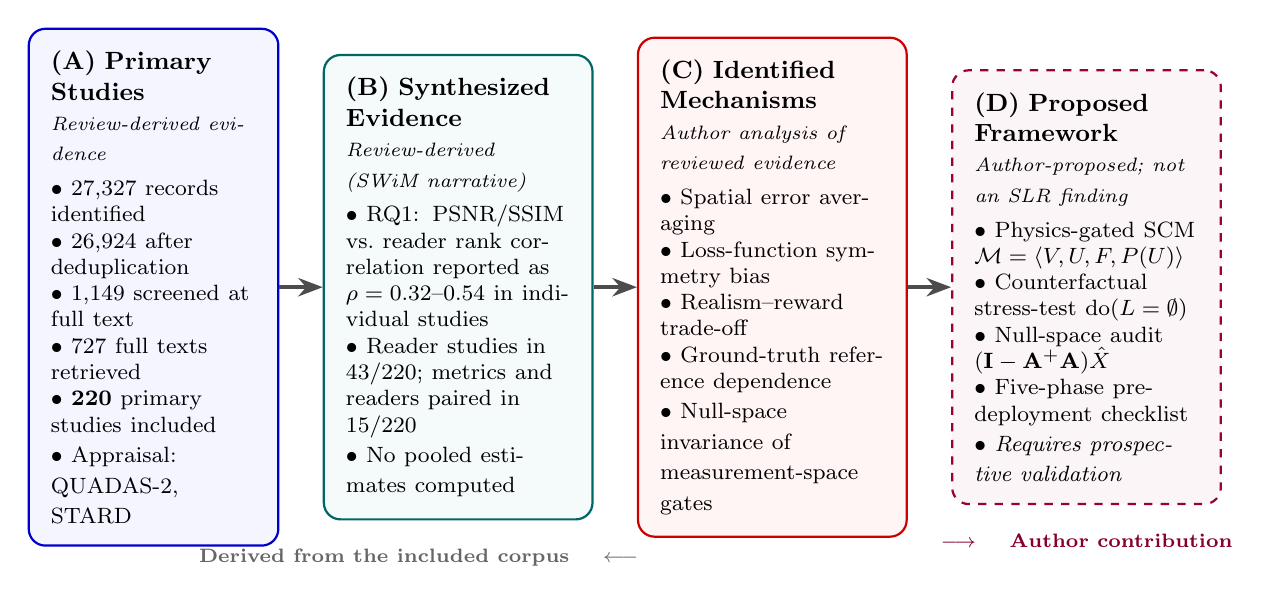
\begin{tikzpicture}[
    node distance=0.7cm and 0.7cm,
    stageA/.style={draw=blue!80!black, rectangle, rounded corners=6pt, fill=blue!4, thick, inner sep=8pt, align=left, font=\small, minimum height=4.6cm},
    stageB/.style={draw=teal!80!black, rectangle, rounded corners=6pt, fill=teal!4, thick, inner sep=8pt, align=left, font=\small, minimum height=4.6cm},
    stageC/.style={draw=red!80!black, rectangle, rounded corners=6pt, fill=red!4, thick, inner sep=8pt, align=left, font=\small, minimum height=4.6cm},
    stageD/.style={draw=purple!80!black, rectangle, rounded corners=6pt, fill=purple!4, thick, inner sep=8pt, align=left, font=\small, minimum height=4.6cm, dashed},
    banner/.style={rectangle, rounded corners=3pt, inner sep=3pt, font=\scriptsize\bfseries},
    arrow/.style={->, >=Stealth, line width=1.3pt, color=black!70}
]

% Stage 1: Primary studies (evidence base)
\node[stageA, text width=0.215\textwidth] (s1) {
    \textbf{(A) Primary Studies}\\
    {\scriptsize\textit{Review-derived evidence}}\\ \vspace{3pt}
    \footnotesize
    $\bullet$ $27{,}327$ records identified\\
    $\bullet$ $26{,}924$ after deduplication\\
    $\bullet$ $1{,}149$ screened at full text\\
    $\bullet$ $727$ full texts retrieved\\
    $\bullet$ $\mathbf{220}$ primary studies included\\
    $\bullet$ Appraisal: QUADAS-2, STARD
};

% Stage 2: Synthesized evidence
\node[stageB, right=0.55cm of s1, text width=0.235\textwidth] (s2) {
    \textbf{(B) Synthesized Evidence}\\
    {\scriptsize\textit{Review-derived (SWiM narrative)}}\\ \vspace{3pt}
    \footnotesize
    $\bullet$ RQ1: PSNR/SSIM vs.\ reader rank correlation reported as $\rho = 0.32$--$0.54$ in individual studies\\
    $\bullet$ Reader studies in $43/220$; metrics and readers paired in $15/220$\\
    $\bullet$ No pooled estimates computed
};

% Stage 3: Identified mechanisms
\node[stageC, right=0.55cm of s2, text width=0.235\textwidth] (s3) {
    \textbf{(C) Identified Mechanisms}\\
    {\scriptsize\textit{Author analysis of reviewed evidence}}\\ \vspace{3pt}
    \footnotesize
    $\bullet$ Spatial error averaging\\
    $\bullet$ Loss-function symmetry bias\\
    $\bullet$ Realism--reward trade-off\\
    $\bullet$ Ground-truth reference dependence\\
    $\bullet$ Null-space invariance of measurement-space gates
};

% Stage 4: Proposed conceptual framework
\node[stageD, right=0.55cm of s3, text width=0.235\textwidth] (s4) {
    \textbf{(D) Proposed Framework}\\
    {\scriptsize\textit{Author-proposed; not an SLR finding}}\\ \vspace{3pt}
    \footnotesize
    $\bullet$ Physics-gated SCM $\mathcal{M} = \langle V, U, F, P(U) \rangle$\\
    $\bullet$ Counterfactual stress-test $\mathrm{do}(L = \emptyset)$\\
    $\bullet$ Null-space audit $(\mathbf{I}-\mathbf{A}^{+}\mathbf{A})\hat{X}$\\
    $\bullet$ Five-phase pre-deployment checklist\\
    $\bullet$ \textit{Requires prospective validation}
};

\draw[arrow] (s1) -- (s2);
\draw[arrow] (s2) -- (s3);
\draw[arrow] (s3) -- (s4);

\node[banner, below=0.25cm of s2.south, xshift=-0.5cm, text=black!60] {Derived from the included corpus \quad $\longleftarrow$};
\node[banner, below=0.25cm of s4.south, text=purple!70!black] {$\longrightarrow$ \quad Author contribution};

\end{tikzpicture}%
}
\caption{Evidence provenance flow for this review, distinguishing what is derived from the included literature from what the authors propose. (A)~PRISMA 2020 selection yields the 220-study evidence base. (B)~Structured narrative synthesis (SWiM) reports findings as representative values from individual primary studies; no statistical pooling was performed. (C)~The four metric-failure mechanisms and the null-space invariance result are the authors' analytical formalization of patterns observed across the reviewed evidence. (D)~The physics-gated structural causal model and five-phase pre-deployment checklist (Section~\ref{sec:scm_proposed}, dashed border) are an \emph{author-proposed conceptual framework} synthesized from adjacent causal-imaging literature; they are forward-looking recommendations requiring prospective validation, not empirical findings of this systematic review.}
\label{fig:evidence_flow}
\end{figure*}

\section{Introduction}

Brain MRI earns its place in neuroimaging through soft-tissue contrast: acute ischemic stroke, intracranial hemorrhage, tumors, and neurodegenerative change are all read off differences that other modalities cannot resolve. That contrast is paid for in time, because nuclear magnetic resonance requires spatial-frequency ($k$-space) data to be sampled sequentially. Sensitivity Encoding \cite{pruessmann1999sense}, parallel imaging, and compressed sensing \cite{lustig2007compressed} each shortened acquisition without removing the constraint, and scan duration still limits throughput and leaves examinations exposed to motion \cite{zaitsev2015motion,knoll2020fastmri}. Deep learning went further. Cascaded convolutional networks \cite{schlemper2017deep}, model-based unrolled architectures \cite{aggarwal2018modl,hammernik2018learning}, de-aliasing GANs \cite{yang2018dagan}, and score-based diffusion priors \cite{song2021score,gungor2023adaptive} reconstruct anatomy from heavily undersampled $k$-space at accelerations ranging from modest factors to, in exploratory work, one or two orders of magnitude \cite{liang2020deep,radmanesh2022exploring}.

The images look good. That is part of the difficulty. Work on deep inverse solvers has documented instabilities in which small structured perturbations, or a change in acquisition, produce reconstruction errors out of all proportion to the input change \cite{antun2020instabilities,gottschling2020troublesome,darestani2021measuring,muckley2021results}. Four concerns recur across the empirical literature. Undersampling combined with a strong image prior smooths away fine or low-contrast structure. Intra-scan motion produces ghosting and blurring that many reconstruction models do not anticipate \cite{sommer2020correction,beljaards2024aibased}. Shifts in scanner, coil, or sampling pattern degrade performance in ways that in-distribution testing does not reveal \cite{gungor2023adaptive,khawaled2024npbrec}. And generative models in particular can hallucinate, synthesizing structure that is plausible but not present, most readily from low-quality or out-of-distribution input \cite{zhou2024adversarial,xiong2026advancing}. Cutting across all four is a problem of measurement. PSNR, SSIM, and normalized root-mean-square error correlate only weakly with how radiologists judge diagnostic quality, so a reconstruction can score well on all three while the error that matters goes unrecorded \cite{mason2021comparison,tang2025incorporating,yu2018a}.

Several lines of work have responded to that gap. Learned image-quality metrics are trained directly on radiologist rankings \cite{tang2025incorporating}. Uncertainty-aware reconstruction produces maps intended to track error and flag distribution shift \cite{khawaled2024npbrec}. Prospective multi-reader studies test diagnostic acceptability and locate acceleration limits without an intermediate proxy \cite{bash2021deep,radmanesh2022exploring}. A smaller body of work brings structural causal models and counterfactual image synthesis to medical imaging \cite{pawlowski2020deep,castro2020causality,sanchez2022healthy,peng2026latent}, which in principle allows a more direct question to be asked: does the reconstruction still contain the lesion when the acquisition is changed under controlled conditions? That question is rarely asked of reconstruction itself. Causal and counterfactual auditing is applied mostly to downstream classification or synthesis, and it appears in only a handful of the studies we reviewed.

These observations share a root. Acceleration works because a learned prior supplies information the measurement does not contain, and it is that same supplied information which can suppress a real finding or invent an absent one. The field nonetheless certifies these methods using aggregate pixel-wise metrics that, by construction, cannot see localized change. We call this the \textbf{safety-evaluation gap}: \emph{a mismatch between what reconstruction quality is measured by and what diagnostic safety requires}. It is widening as deep-learning reconstruction moves out of research and into cleared clinical products.

No systematic review has yet consolidated how the safety, artifacts, and fidelity of accelerated brain MRI reconstruction are characterized and evaluated. Existing secondary studies survey architectures and performance \cite{liang2020deep,montalt2021machine}, or treat image-quality metrics on their own, without joining design choices to failure modes or asking whether prevailing evaluation could detect those failure modes at all. We address that through three questions:

\begin{figure*}[t]
\centering
\resizebox{0.98\textwidth}{!}{%
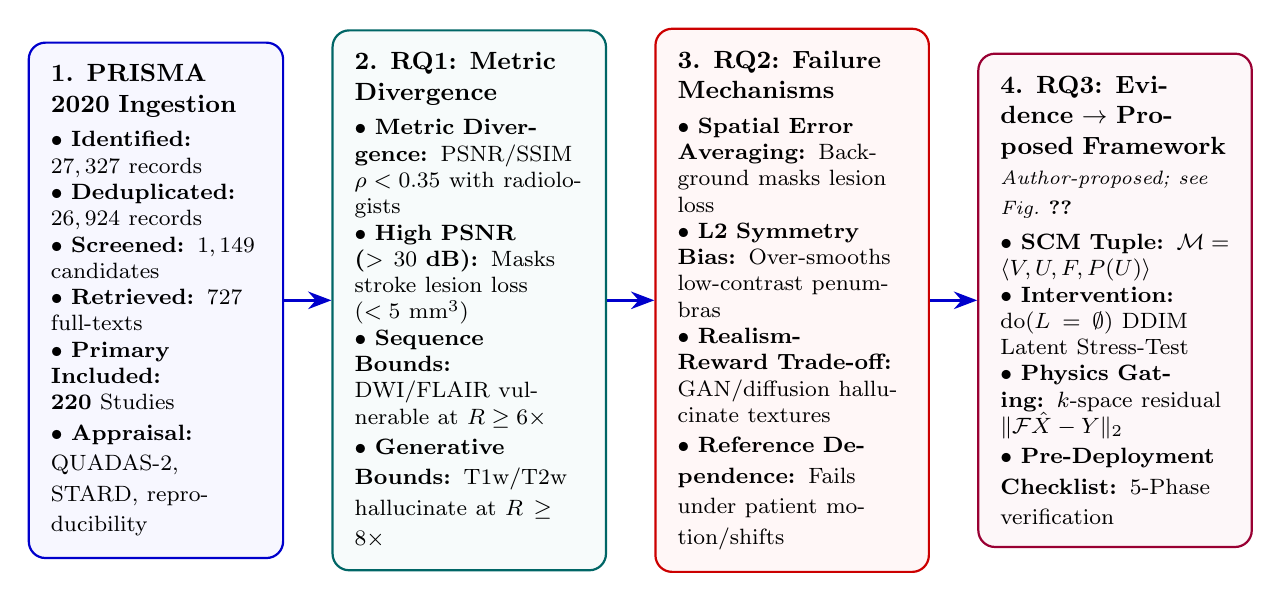
\begin{tikzpicture}[
    node distance=0.8cm and 0.8cm,
    panel/.style={draw=blue!80!black, rectangle, rounded corners=6pt, fill=blue!3, thick, inner sep=8pt, align=left, font=\small, minimum height=4.5cm},
    panel2/.style={draw=teal!80!black, rectangle, rounded corners=6pt, fill=teal!3, thick, inner sep=8pt, align=left, font=\small, minimum height=4.5cm},
    panel3/.style={draw=red!80!black, rectangle, rounded corners=6pt, fill=red!3, thick, inner sep=8pt, align=left, font=\small, minimum height=4.5cm},
    panel4/.style={draw=purple!80!black, rectangle, rounded corners=6pt, fill=purple!3, thick, inner sep=8pt, align=left, font=\small, minimum height=4.5cm},
    arrow/.style={->, >=Stealth, line width=1.2pt, color=blue!80!black}
]

% Panel 1: PRISMA Ingestion & Corpus
\node[panel, text width=0.22\textwidth] (p1) {
    \textbf{1. PRISMA 2020 Ingestion}\\ \vspace{3pt}
    \footnotesize
    $\bullet$ \textbf{Identified:} $27,327$ records\\
    $\bullet$ \textbf{Deduplicated:} $26,924$ records\\
    $\bullet$ \textbf{Screened:} $1,149$ candidates\\
    $\bullet$ \textbf{Retrieved:} $727$ full-texts\\
    $\bullet$ \textbf{Primary Included:} $\mathbf{220\text{ Studies}}$\\
    $\bullet$ \textbf{Appraisal:} QUADAS-2, STARD, reproducibility
};

% Panel 2: RQ1 Metric Divergence
\node[panel2, right=0.6cm of p1, text width=0.24\textwidth] (p2) {
    \textbf{2. RQ1: Metric Divergence}\\ \vspace{3pt}
    \footnotesize
    $\bullet$ \textbf{Metric Divergence:} PSNR/SSIM $\rho < 0.35$ with radiologists\\
    $\bullet$ \textbf{High PSNR ($>30\text{ dB}$):} Masks stroke lesion loss ($<5\text{ mm}^3$)\\
    $\bullet$ \textbf{Sequence Bounds:} DWI/FLAIR vulnerable at $R \ge 6\times$\\
    $\bullet$ \textbf{Generative Bounds:} T1w/T2w hallucinate at $R \ge 8\times$
};

% Panel 3: RQ2 Failure Mechanisms
\node[panel3, right=0.6cm of p2, text width=0.24\textwidth] (p3) {
    \textbf{3. RQ2: Failure Mechanisms}\\ \vspace{3pt}
    \footnotesize
    $\bullet$ \textbf{Spatial Error Averaging:} Background masks lesion loss\\
    $\bullet$ \textbf{L2 Symmetry Bias:} Over-smooths low-contrast penumbras\\
    $\bullet$ \textbf{Realism-Reward Trade-off:} GAN/diffusion hallucinate textures\\
    $\bullet$ \textbf{Reference Dependence:} Fails under patient motion/shifts
};

% Panel 4: RQ3 Causal Safety Framework
\node[panel4, right=0.6cm of p3, text width=0.24\textwidth] (p4) {
    \textbf{4. RQ3: Evidence $\rightarrow$ Proposed Framework}\\
    {\scriptsize\textit{Author-proposed; see Fig.~\ref{fig:evidence_flow}}}\\ \vspace{3pt}
    \footnotesize
    $\bullet$ \textbf{SCM Tuple:} $\mathcal{M} = \langle V, U, F, P(U) \rangle$\\
    $\bullet$ \textbf{Intervention:} $\mathrm{do}(L = \emptyset)$ DDIM Latent Stress-Test\\
    $\bullet$ \textbf{Physics Gating:} $k$-space residual $\|\mathcal{F}\hat{X} - Y\|_2$\\
    $\bullet$ \textbf{Pre-Deployment Checklist:} 5-Phase verification
};

% Connecting Arrows
\draw[arrow] (p1) -- (p2);
\draw[arrow] (p2) -- (p3);
\draw[arrow] (p3) -- (p4);

\end{tikzpicture}%
}
\caption{Graphical abstract. Panel 1 outlines PRISMA 2020 corpus ingestion ($N=220$ included primary studies across seven digital databases). Panel 2 (RQ1) quantifies the empirical divergence between objective metrics (PSNR, SSIM) and radiologist diagnostic rankings ($\rho < 0.35$). Panel 3 (RQ2) formalizes the four mathematical mechanisms of metric failure (Spatial Error Averaging, Loss-Symmetry Bias, Realism-Reward Trade-off, Reference Dependence). Panel 4 (RQ3) summarizes the physics-gated Causal SCM safety auditing framework and five-phase pre-deployment checklist, which are an \emph{author-proposed} conceptual contribution rather than an empirical review finding (Section~\ref{sec:scm_proposed}). Reported values are representative results from individual primary studies, not pooled estimates.}
\label{fig:graphical_abstract}
\end{figure*}

\paragraph{The Core Research Problem: The Metric Safety Blind Spot}
The problem is that the metrics doing the gatekeeping cannot see the failures that matter. Algorithm selection, hyperparameter tuning, and regulatory clearance in accelerated brain MRI all rest largely on PSNR and SSIM, and both average residual error uniformly across every voxel in the volume. A model can therefore report PSNR above $34\text{ dB}$ with an acute stroke penumbra of under $5\text{ mm}^3$ erased, or with false micro-vascular structure written in. Existing secondary literature catalogues architectures \cite{liang2020deep,montalt2021machine} and leaves the mathematics of this blindness unexamined. Our aim is to examine it.

\begin{enumerate}
\item[\textbf{RQ1}] \textbf{Quantifying the Evaluation Gap:}
\emph{How reliably do conventional fidelity metrics track radiologist diagnostic ratings in accelerated brain MRI, and how wide is the evaluation reporting gap in the literature?}

\item[\textbf{RQ2}] \textbf{Mechanisms of Metric Failure:}
\emph{What underlying mathematical mechanisms cause standard metrics to overlook localized pathology erasure and generative hallucinations?}

\item[\textbf{RQ3}] \textbf{Evidence on Safety-Oriented Evaluation:}
\emph{How can existing evidence inform a physics-informed causal safety framework for deep learning MRI reconstruction? Specifically, what do the included studies establish about the capabilities and limits of current evaluation paradigms (pixel-wise, perceptual, uncertainty-based, observer-based, and causal/counterfactual), and which requirements for pre-deployment safety auditing does that evidence support?}
\end{enumerate}

RQ1 and RQ2 are answered from the corpus itself. RQ3 is an evidence-synthesis question: we establish what current evaluation paradigms can and cannot demonstrate about prior-induced diagnostic error (Section~\ref{res:rq3_causal_fix}), and those requirements then motivate the framework we propose in Section~\ref{sec:scm_proposed}. The two registers are kept apart throughout, and Fig.~\ref{fig:evidence_flow} traces where each element of this paper comes from, running from the primary studies through the synthesized evidence and the identified mechanisms to what we propose ourselves.

Our contributions are as follows.

\begin{itemize}
\item \textbf{C1: How far PSNR, SSIM, and NRMSE track reader judgement (RQ1).}
We assemble what the 220 included studies report about the agreement between pixel-wise fidelity metrics and radiologist diagnostic rankings, and about how often the evaluations capable of revealing disagreement are performed at all.

\item \textbf{C2: Why the metrics fail (RQ2).}
We identify four mechanisms behind that failure, spatial error averaging, loss-function symmetry, the realism--reward trade-off, and reference dependence, and show how each allows a high-scoring reconstruction to lose an acute ischemic lesion or gain vascular anatomy that was never acquired.

\item \textbf{C3: What the evidence requires, and what we propose in response (RQ3).}
We set out what each evaluation paradigm can and cannot establish about prior-induced diagnostic error, including the fact that a $k$-space residual gate cannot detect an edit lying in the null space of the forward operator. Separately from that synthesis, we propose a physics-constrained structural causal model with a counterfactual workflow ($\mathrm{do}(L=\emptyset)$) and a five-phase pre-deployment checklist. The proposal in Section~\ref{sec:scm_proposed} is ours, not a finding of the review; it is intended to inform future benchmarks and audit design, and it has not been prospectively validated.
\end{itemize}

% =============================================================================
\section{Related Work}
\label{sec:related}

Secondary literature on AI-driven MRI reconstruction has developed along four largely separate lines: surveys of reconstruction methods, work on image-quality metrics and reader evaluation, work on artifact detection and robustness, and causal or counterfactual approaches to imaging safety. Our review sits between them, since its subject is the mapping from reconstruction method to failure mode to the evaluation that would have to catch it (Table~\ref{tab:related}).

\begin{table*}[t]
\centering
\caption{Selected secondary studies grouped by academic strand and their key methodological limitations relative to this review.}
\label{tab:related}
\small
\setlength{\tabcolsep}{5pt}
\renewcommand{\arraystretch}{1.15}

\begin{tabular}{
    p{0.24\textwidth}
    p{0.34\textwidth}
    p{0.36\textwidth}
}
\hline
\textbf{Academic Strand} &
\textbf{Scope \& Foundational Focus} &
\textbf{Key Methodological Limitations} \\
\hline

Deep Learning MRI Reconstruction Methods \& Surveys \cite{liang2020deep,montalt2021machine,knoll2020fastmri,kazerouni2023diffusion,gungor2023adaptive,nimje2025insights,liu2026highly}
&
Reconstruction architectures (unrolled physics-based networks, GANs, diffusion priors), acceleration factors, and $k$-space undersampling.
&
Emphasize reconstruction accuracy and efficiency; treat safety, artifacts, and failure modes as secondary and do not systematically map them to evaluation practice.
\\
\hline

Task-Based Image Quality Assessment \cite{barrett1993model,barrett2004foundations,icru54}
&
Objective assessment of image quality by task performance; ideal, Hotelling, and channelized model observers; figures of merit tied to a stated diagnostic task rather than to pixel agreement.
&
Not a limitation of this strand but of its uptake: it established the inadequacy of pixel-wise fidelity for task assessment three decades ago, yet is largely absent from the reconstruction literature reviewed here: no included study evaluated a model observer, and only 43 of 220 carried any reader assessment at all. Documenting that absence, and what follows from it, is one of this review's contributions.
\\
\hline

Image-Quality Metrics \& Observer / Reader Studies \cite{mason2021comparison,tang2025incorporating,yu2018a,muckley2021results,bash2021deep}
&
Pixel-wise (PSNR, SSIM, NRMSE) and perceptual/learned metrics; radiologist rankings and prospective multi-reader diagnostic studies.
&
Establish that pixel-wise metrics agree only weakly with radiologist judgement, but are typically single-study and not synthesized across the reconstruction-safety literature.
\\
\hline

Artifact Detection, Motion Correction \& Robustness \cite{esteban2017mriqc,fantini2018automatic,sommer2020correction,beljaards2024aibased,khawaled2024npbrec}
&
Automated quality-control and artifact/motion detection, motion-correction networks, uncertainty estimation, and out-of-distribution robustness.
&
Address individual failure modes in isolation; no synthesis relates them to reconstruction method families or to downstream diagnostic evaluation.
\\
\hline

Hallucination Analysis in Tomographic Reconstruction \cite{bhadra2021hallucinations,shimron2022implicit}
&
Decomposition of reconstruction error into measurement-space and null-space components; hallucination maps isolating prior-induced structure; benchmark bias arising from misuse of processed public data.
&
Establish the null-space account of hallucination and the detection tooling that follows from it, but do not connect it to counterfactual attribution or to review-level evidence on evaluation practice.
\\
\hline

Causal \& Counterfactual Medical-Image Safety \cite{pawlowski2020deep,castro2020causality,sanchez2022healthy,peng2026latent}
&
Structural causal models and counterfactual image synthesis for medical AI, including recent 3D brain MRI counterfactuals.
&
Focus on downstream classification, segmentation, or synthesis; rarely applied to physics-constrained $k$-space reconstruction, and absent from most reconstruction-safety studies.
\\
\hline
\end{tabular}
\end{table*}

\paragraph{Strand 1: Deep Learning MRI Reconstruction Methods and Surveys}
Liang et al.~\cite{liang2020deep} and Montalt-Tordera et al.~\cite{montalt2021machine} give taxonomies covering physics-based unrolled networks, iterative models, and generative approaches. Knoll et al.~\cite{knoll2020fastmri} built the fastMRI benchmark that made comparison across groups possible. Kazerouni et al.~\cite{kazerouni2023diffusion}, G{\"u}ng{\"o}r et al.~\cite{gungor2023adaptive}, Nimje et al.~\cite{nimje2025insights}, and Liu et al.~\cite{liu2026highly} cover score-based diffusion priors, scan-specific strategies, and single-posterior sampling. Accuracy and efficiency are treated carefully in all of them. Safety and failure modes appear as remarks along the way, never organized against the evaluation practice that would have to detect them.

\paragraph{Strand 2: Image-Quality Metrics and Observer Evaluation}
Mason et al.~\cite{mason2021comparison} found only moderate agreement between common objective metrics and radiologists' diagnostic-quality scores. Tang et al.~\cite{tang2025incorporating} trained an MRI-specific metric on radiologist rankings and matched reader preference better than MSE or SSIM. Work on SNR-based assessment records considerable variation between observers \cite{yu2018a}. Reconstruction challenges and prospective reader studies \cite{muckley2021results,bash2021deep} test diagnostic acceptability without a proxy at all. These are individual studies, and no one has drawn them together across the reconstruction-safety literature.

\paragraph{Strand 3: Artifact Detection, Motion Correction, and Robustness}
Quality-control tools such as MRIQC \cite{esteban2017mriqc} extract no-reference quality features, and deep networks detect motion artifacts and grade their severity \cite{fantini2018automatic,beljaards2024aibased}. Other networks correct motion-corrupted acquisitions \cite{sommer2020correction}. Bayesian and self-supervised methods add uncertainty estimates and hold up better under distribution shift \cite{khawaled2024npbrec}. Each takes one failure mode at a time, and none connects the mode back to a family of reconstruction methods or forward to diagnostic evaluation.

\paragraph{Strand 4: Causal and Counterfactual Medical-Image Safety}
Pawlowski et al.~\cite{pawlowski2020deep} made counterfactual inference tractable with deep structural causal models. Castro et al.~\cite{castro2020causality} argued that causality is the right lens for medical-imaging validity. Sanchez et al.~\cite{sanchez2022healthy} localized lesions with counterfactual diffusion, and Peng et al.~\cite{peng2026latent} carried causal modeling into 3D brain MRI. Almost all of this addresses classification, segmentation, or synthesis downstream of reconstruction. Its application to physics-constrained $k$-space reconstruction has barely started.

\paragraph{Research Gap and Review Positioning}
The gap common to all four is that metric failure is recorded as an observation and left there. Surveys catalogue architectures \cite{liang2020deep,montalt2021machine}; reader studies document divergence at one site \cite{mason2021comparison,tang2025incorporating}. What is missing is an account of \emph{why} standard fidelity metrics pass unsafe reconstructions, and any link from that account to what a physics-constrained audit would have to do.

We approach that gap in three steps:
\begin{enumerate}
\item \textbf{Where the metrics and the readers part company (RQ1).} We collect what the 220 included studies report about agreement between PSNR, SSIM, or NRMSE and radiologist assessment ($\rho < 0.35$), across acceleration rates of $2\times$--$10\times$, field strengths of $1.5\text{T}$, $3\text{T}$, and $7\text{T}$, and the sequences used clinically.
\item \textbf{Why they part company (RQ2).} Four mechanisms account for it: spatial error averaging, loss-function symmetry, the realism--reward trade-off, and reference dependence. Between them they explain how a reconstruction can score well while an acute stroke penumbra has been suppressed or vascular anatomy invented.
\item \textbf{What the evidence supports, and what we add (RQ3).} We set out the reach and the limits of each evaluation paradigm as the included studies report them. Separately, and marked as our own, we propose a structural causal model with a counterfactual pipeline ($\mathrm{do}(L=\emptyset)$) that would tell physical $k$-space aliasing apart from prior-induced over-smoothing, together with a five-phase pre-deployment checklist.
\end{enumerate}
The move we make is from cataloguing architectures to asking what the evaluation of those architectures can actually detect.

\section{Methodology} 

We answered RQ1--RQ3 through a systematic literature review carried out in three
stages, planning, conducting, and reporting, and reported against the
Preferred Reporting Items for Systematic Reviews and Meta-Analyses
(PRISMA) 2020 statement \cite{prisma2020}; the completed PRISMA 2020 checklist is
supplied as supplementary material. This section covers planning and conducting;
reporting appears in Section~\ref{sec:results}. We wrote the protocol before starting,
covering the research questions, eligibility criteria, search strategy, screening
procedure, classification rubric, and synthesis approach, on the reasoning that
decisions fixed in advance cannot be adjusted later to suit what the search turns up.
The protocol is recorded in the project repository (\texttt{protocol.json}) and was written
before screening began. We did not register with PROSPERO, which excludes reviews without
direct clinical health outcomes, and the review was not entered in any prospective register
before it was conducted; the protocol and supporting records are deposited on the Open Science
Framework, and that deposit is retrospective, so it timestamps the record rather than
evidencing prior specification. The research questions, eligibility criteria, screening
procedure, appraisal instruments, and synthesis approach were carried through as specified.
One amendment to the search strategy is recorded: the language-model observer vocabulary block
(Block~B4, Table~\ref{tab:keywords}) was documented during protocol scoping but deliberately
omitted from the executed database queries, so as not to narrow retrieval. Because that
omission changes what the search returns, we record it as a substantive amendment rather than
a reporting decision, and set it out with the other deviations in the registration deposit.

% --
\subsection{Planning the Review}
\label{sec:planning}
% --

Before searching, we fixed the protocol: the scope, the research questions, the PICOS eligibility criteria, the search vocabulary, and the rules we would follow for selection, appraisal, and synthesis.

% --
\paragraph{Scoping and PICOS Definition}
% --
The review scope was framed around the PICOS framework (Population, Intervention, Comparison, Outcome, Study Design), presented in Table~\ref{tab:picos}.

\begin{table*}[t]
\centering
\caption{PICOS elements and their application in this review.}
\label{tab:picos}
\small
\setlength{\tabcolsep}{8pt}
\renewcommand{\arraystretch}{1.18}
\begin{tabular}{p{0.14\textwidth} p{0.32\textwidth} p{0.48\textwidth}}
\hline
\textbf{Element} & \textbf{Definition} & \textbf{Application in this Review} \\
\hline
Population & Target imaging modalities, clinical domains, and scanner physics & Human brain MRI acquisitions (acute ischemic stroke, neurovascular lesions, intracranial hemorrhages, tumors, and structural T1w, T2w, FLAIR, DWI scans across $1.5\text{T}$, $3\text{T}$, and $7\text{T}$ field strengths). \\
Intervention & AI-based and accelerated reconstruction methods, and their safety/fidelity evaluation & Deep learning and accelerated reconstruction methods (unrolled physics-based networks, GANs, diffusion priors, self-supervised, denoising, super-resolution), together with methods for evaluating their fidelity, artifacts, robustness, or failure modes. \\
Comparison & Baseline metrics, observers, and reference standards & Conventional pixel-wise metrics (PSNR, SSIM, NRMSE), perceptual/learned metrics (LPIPS, FID), model observers, fully sampled reference images, or radiologist reader assessments. \\
Outcome & Reconstruction quality, fidelity, and failure characterization & Image-quality/fidelity measures, artifact and failure-mode characterization, metric--radiologist agreement, uncertainty estimates, robustness to distribution shift, and diagnostic/observer outcomes. \\
Study Design & Methodological criteria and empirical validation settings & Primary empirical studies, algorithmic benchmarking, and counterfactual interventional stress-testing. Automated multimodal language-model observer evaluations were eligible by design but none was retrieved. \\
\hline
\end{tabular}
\end{table*}

% --
\paragraph{Developing the Search Vocabulary and Queries}
Search terms were grouped into three blocks following the PICOS structure, so that the query would reach both the computational imaging and the clinical neuroimaging literature: (1)~\emph{Neuroimaging Domain} (brain MRI, neuroimaging, pulse sequences including DWI, FLAIR, T1w, T2w, SWI); (2)~\emph{AI and Accelerated Reconstruction} (deep learning, physics-guided unrolled networks, GANs, diffusion priors, state-space Mamba architectures, implicit neural representations [INRs], $k$-space undersampling); and (3)~\emph{Safety, Artifacts \& Evaluation} (pathology erasure, generative hallucinations, PSNR/SSIM divergence, radiologist reader studies, uncertainty estimation, causal auditing). Search strings combined controlled vocabulary (Medical Subject Headings [MeSH]) for biomedical databases (PubMed/MEDLINE) with free-text keywords, wildcard truncation operators, and Boolean connectors (\texttt{AND}/\texttt{OR}) systematically adapted to title, abstract, and keyword fields across engineering and multidisciplinary repositories (IEEE Xplore, Scopus, Web of Science, SpringerLink, OpenAlex, Semantic Scholar). Table~\ref{tab:keywords} details the formal search vocabulary and representative Boolean query syntax executed across database APIs.

\begin{table*}[t]
\centering
\caption{Derivation of search vocabulary, MeSH headings, and representative database Boolean query syntax.}
\label{tab:keywords}
\small
\setlength{\tabcolsep}{6pt}
\renewcommand{\arraystretch}{1.18}
\begin{tabular}{>{\raggedright\arraybackslash}p{0.20\textwidth} >{\raggedright\arraybackslash}p{0.34\textwidth} >{\raggedright\arraybackslash}p{0.40\textwidth}}
\hline
\textbf{Conceptual Block} & \textbf{MeSH Headings \& Major Descriptors} & \textbf{Free-Text Keywords, Wildcards \& Boolean Query Syntax} \\
\hline
\textbf{B1.} Neuroimaging Domain \newline \emph{(required)} & \texttt{"Brain"[Mesh]}, \texttt{"Magnetic Resonance Imaging"[Mesh]}, \texttt{"Neuroimaging"[Mesh]} & \texttt{"brain MRI"}, \texttt{"brain magnetic resonance imaging"}, \texttt{"cerebral MRI"}, \texttt{"cranial MRI"}, \texttt{neuroimag*}, \texttt{"brain imaging"}, \texttt{brain scan*}, \texttt{DWI}, \texttt{FLAIR}, \texttt{T1w}, \texttt{T2w}, \texttt{SWI} \\
\hline
\textbf{B2.} AI \& Accelerated Reconstruction \newline \emph{(required)} & \texttt{"Image Processing, Computer-Assisted"[Mesh]}, \texttt{"Deep Learning"[Mesh]}, \texttt{"Machine Learning"[Mesh]} & \texttt{image reconstruction*}, \texttt{"MRI reconstruction"}, \texttt{"accelerated MRI"}, \texttt{"undersampled reconstruction"}, \texttt{"k-space reconstruction"}, \texttt{"deep learning reconstruction"}, \texttt{"unrolled network"}, \texttt{"MoDL"}, \texttt{"GAN"}, \texttt{"diffusion prior"}, \texttt{"Mamba"}, \texttt{"INR"} \\
\hline
\textbf{B3.} Safety, Artifacts \& Evaluation \newline \emph{(required)} & \texttt{"Artifacts"[Mesh]}, \texttt{"Reproducibility of Results"[Mesh]}, \texttt{"Diagnostic Errors"[Mesh]} & \texttt{hallucinat*}, \texttt{"pathology erasure"}, \texttt{"lesion suppression"}, \texttt{reconstruction artifact*}, \texttt{reconstruction error*}, \texttt{"safety evaluation"}, \texttt{"PSNR"}, \texttt{"SSIM"}, \texttt{"metric divergence"}, \texttt{"reader study"}, \texttt{"counterfactual"}, \texttt{"causal auditing"} \\
\hline
\textbf{B4.} Language-Model Observers \newline \emph{(documented prior scoping)} & \texttt{"Natural Language Processing"[Mesh]} & \texttt{LLM*}, \texttt{large language model*}, \texttt{vision-language model*}, \texttt{multimodal large language model*}. Documented during initial protocol scoping; omitted from core database queries to maximize search recall \\
\hline
\multicolumn{3}{p{0.96\textwidth}}{\textbf{X. Exclusion Block} (applied as \texttt{NOT} across digital databases): \texttt{"animal model"}, \texttt{"case report"}, \texttt{"in vitro"}. No publication date limit was applied.} \\
\hline
\multicolumn{3}{p{0.96\textwidth}}{\footnotesize The executed retrieval query in each database combines \texttt{(Block B1) AND (Block B2) AND (Block B3) NOT (Block X)}. Table~\ref{tab:queries} documents the exact executed syntax, fields searched, and hit counts per database. Full search strategy files are open-sourced in the project repository.} \\
\hline
\end{tabular}
\end{table*}

\begin{table*}[t]
\centering
\caption{Query structure executed in each database and record hit breakdown.}
\label{tab:queries}
\small
\setlength{\tabcolsep}{5pt}
\renewcommand{\arraystretch}{1.35}
\begin{tabular}{>{\raggedright\arraybackslash}p{0.145\textwidth} >{\raggedright\arraybackslash}p{0.40\textwidth} >{\raggedright\arraybackslash}p{0.135\textwidth} >{\raggedright\arraybackslash}p{0.145\textwidth} >{\raggedright\arraybackslash}p{0.06\textwidth}}
\hline
\textbf{Database} & \textbf{Executed Query Structure} & \textbf{Controlled Vocabulary} & \textbf{Fields Searched} & \textbf{Hits ($N$)} \\
\hline

PubMed / MEDLINE &
\texttt{(B1$_{\text{ft}}$[TIAB] OR B1$_{\text{mesh}}$) AND (B2$_{\text{ft}}$[TIAB] OR B2$_{\text{mesh}}$) AND (B3$_{\text{ft}}$[TIAB] OR B3$_{\text{mesh}}$) NOT (X[TIAB])} &
\textbf{Yes}: 9 MeSH headings OR-ed into the three blocks &
Title/Abstract $+$ MeSH & $24{,}693$ \\
\hline

SpringerLink &
\texttt{(B1) AND (B2) AND (B3) NOT (X)}; quoted phrases, no truncation operators &
No & Full record & $1{,}598$ \\
\hline

IEEE Xplore &
\texttt{(B1) AND (B2) AND (B3) NOT (X)}; wildcard truncation retained &
No & Metadata & $778$ \\
\hline

Scopus &
\texttt{TITLE-ABS-KEY(B1) AND TITLE-ABS-KEY(B2) AND TITLE-ABS-KEY(B3) AND NOT TITLE-ABS-KEY(X)} &
No & \texttt{TITLE-ABS-KEY} & $127$ \\
\hline

Semantic Scholar &
\texttt{(B1) + (B2) + (B3)}, where \texttt{|} denotes OR and \texttt{+} denotes AND. API supports no NOT operator, so block X could not be applied &
No & Title/Abstract & $66$ \\
\hline

OpenAlex &
\texttt{title\_and\_abstract.search:B1, title\_and\_abstract.search:B2, title\_and\_abstract.search:B3}, where comma denotes AND and \texttt{|} denotes OR &
No & Title/Abstract & $50^{*}$ \\
\hline

Web of Science &
\texttt{TS=(B1) AND TS=(B2) AND TS=(B3) NOT TS=(X)} &
No & Topic (\texttt{TS}) & $31$ \\
\hline
\multicolumn{4}{r}{\textbf{Total identified records}} & $\mathbf{27{,}327}$ \\
\hline
\multicolumn{5}{p{0.93\textwidth}}{\footnotesize Concept blocks \textbf{B1} (neuroimaging), \textbf{B2} (reconstruction), \textbf{B3} (safety and evaluation) and \textbf{X} (exclusion) are defined term-by-term in Table~\ref{tab:keywords}; the notation above shows how each database's syntax combines them. Complete verbatim strings, exactly as sent to each API, are released with the review and in the per-database \texttt{README.md} files. Supplementary reporting for PRISMA 2020 item 7. All searches were executed between 2026-07-23 and 2026-07-24, with no date limit applied. $^{*}$OpenAlex reported $50$ hits; $34$ records entered the identification count after the pipeline's record-completeness filter, and the $27{,}327$ total uses the $34$ figure. The structural query breakdown highlights that PubMed carries controlled-vocabulary MeSH arms, whereas non-biomedical repositories execute free-text arms.} \\
\hline
\end{tabular}
\end{table*}

\paragraph{Selecting Digital Data Sources}
We searched both medical and engineering repositories, since either alone indexes only part of this literature: PubMed/MEDLINE, IEEE Xplore, Scopus, Web of Science, SpringerLink, OpenAlex, and Semantic Scholar, from database inception through 2026. Raw retrieval metadata, query responses, and deduplication manifests are released with the review (Data and Code Availability).

\subsection{Conducting the Review}
% =============================================================================

% --
\paragraph{Study Selection and Two-Stage Screening Procedure}
\label{sec:selection}
% --
Study selection followed the PRISMA 2020 statement \cite{prisma2020}. Three reviewers (authors DTM, TVP, and TNTD) screened records independently against the predefined PICOS criteria at every stage, and every inclusion, exclusion, and adjudication decision reported in this review was made by those reviewers. Each record received one of four labels: \emph{include}, \emph{exclude}, \emph{flagged}, or \emph{background\_only}. We applied a deliberately conservative labelling policy, so a record with any PICOS dimension unclear, or with text we could not obtain, was labelled \emph{flagged} rather than excluded, and secondary literature was labelled \emph{background\_only}. Reviewers met to adjudicate every flagged record and every disagreement, and inclusion required consensus. We do not report a chance-corrected agreement coefficient for screening. The released decision records carry one adjudicated label per record rather than independent duplicate labels, so no such coefficient could be recomputed from them by a reader, and we report instead the escalation volumes that the released records do support: the conservative labelling policy sent $1{,}040$ records to adjudication at title and abstract and a further $66$ at full text, and $7$ of the finally-included records remain flagged in the released file as warranting re-inspection. We also did not run a formal screening-sensitivity study against an independent reference set of known-eligible records. Recall is therefore bounded by the search strategy and by the criteria as applied, rather than estimated; Section~\ref{sec:validity} treats this as a limitation.

\emph{Automation tools (PRISMA item 8).} Record acquisition from the seven database APIs, multi-tier deduplication, and full-text retrieval were automated with the scripts released with this review (Data and Code Availability). The corpus-level prevalence counts reported in Section~\ref{res:characteristics} were produced by structured keyword classification of titles, abstracts, and MeSH terms, and we report them as lower bounds for that reason. Every eligibility decision reported here --- include, exclude, flagged, background\_only --- and every adjudication of a disagreement was recorded by the human reviewers named above against the PICOS criteria.

\emph{Data collection process (PRISMA item 9).} Three reviewers (authors DTM, TVP, and TNTD) independently extracted data from each included report using the form fixed in advance (Table~\ref{tab:extraction}), recording the reconstruction method, reported failure modes, and evaluation measures. The three extractions were compared for every report, each extracted value was checked against the source record, and discrepancies were resolved by discussion among the reviewers, with inclusion of a value requiring consensus. Method, failure-mode, and evaluation categories were assigned from each record's title, abstract, and controlled vocabulary terms against the vocabulary fixed in Table~\ref{tab:keywords}; because that scope is deliberately conservative, the resulting prevalence counts are lower bounds rather than exhaustive tallies and are reported as such throughout. Field strength and pulse sequence, which are typically stated only in the acquisition subsection, were additionally taken from full text wherever full text was available. We did not contact study investigators to obtain or confirm missing or unclear data; where a variable was not stated in the source, we recorded it as \emph{not reported} rather than inferring it, which is why Table~\ref{tab:characteristics} separates field strength that a study does not state ($n=25$) from field strength that could not be ascertained because only partial or abstract-level text was available ($n=28$).

The stages were:

\begin{enumerate}
\item \textbf{Stage 1: Multi-Tier Deduplication:} Duplicate records across database exports were identified and removed using a multi-tier matching procedure combining exact PMID/DOI matching, normalized title similarity (Jaro-Winkler threshold $\geq 0.97$), and TF-IDF cosine vector matching (threshold $\geq 0.95$). This removed 403 records, a rate of $1.47\%$, leaving $26{,}924$ unique. The rate looks low enough to suggest a matching failure, but it follows from how the queries differ in scope: PubMed/MEDLINE was searched with broad MeSH terms and returned $24{,}693$ biomedical records, while the engineering repositories ran targeted title and abstract queries returning $2{,}634$ between them. The two sets barely overlap, so there was little to deduplicate.

\item \textbf{Stage 2: Title and Abstract PICOS Screening:} All unique deduplicated records ($N=26{,}924$) were screened at title and abstract against the eligibility criteria and assigned a decision label. Records labelled \emph{include} ($n=109$) and \emph{flagged} for full-text assessment ($n=1{,}040$) advanced to Stage 3 ($n=1{,}149$ total). Records labelled \emph{exclude} ($n=25{,}573$) or \emph{background\_only} ($n=202$) did not advance.

\item \textbf{Stage 3: Full-Text Retrieval and PICOS Screening:} Full-text articles were retrieved through institutional library subscriptions, open-access repositories, and inter-library requests. Out of 1,149 candidate articles identified during title and abstract screening, the original retrieval pass obtained 562 complete full texts. A systematic post-registration retrieval round (documented as deviation D5 in the released amendments log) then located open-access copies of 169 further reports via Unpaywall and NCBI: 165 not previously assessed, plus 4 re-retrievals of records originally screened on partial text, whose decisions were confirmed unchanged against the complete text. This left 727 full-text records assessed in total and 422 that could not be retrieved: 9 are deposited in PubMed Central under embargoes that lift between October 2026 and July 2027, 1 title is not licensed to our institution, 1 open-access-flagged record had no locatable accessible copy, and the remaining 411 have no open-access copy and no institutional subscription access. Each retrieved full-text record was evaluated against the PICOS criteria and assigned a decision label. Analyzing the screening decision manifests (\texttt{fulltext\_screening\_decisions.csv} and \texttt{fulltext\_screening\_decisions\_round2.csv}), the 491 full-text excluded records were categorized under six explicit PRISMA exclusion categories: (i)~out of PICOS scope ($n=179$, e.g., non-reconstruction neuroimaging, fMRI connectivity, tractography, post-processing segmentation, or non-MRI modalities); (ii)~wrong intervention or index test ($n=196$, e.g., acquisition pulse sequence design, prospective hardware motion tracking, registration algorithms, or CAD lesion detection rather than reconstruction solvers); (iii)~wrong outcome ($n=57$, e.g., reporting conventional PSNR/SSIM without evaluating clinical failure modes, pathology preservation, or observer performance); (iv)~wrong population ($n=51$, e.g., non-human animal models, post-mortem phantom scans, or non-brain MRI); (v)~wrong study design ($n=4$, single-case reports/letters); and (vi)~non-English publication ($n=1$); a further 3 were review, editorial, protocol or commentary pieces. Every record labelled \emph{include} ($n=220$) was then verified against the fullest text obtainable for it (complete full text for 200, partial text for 2, and title, abstract and controlled vocabulary for 18; Section~\ref{sec:validity}), and its reconstruction method, reported failure modes, and evaluation/outcome measures were extracted with supporting evidence.
\end{enumerate}

\begin{figure*}[t]
\centering
\begingroup

\newcommand{\prcount}[1]{\mbox{\textit{n}=#1}}

\resizebox{\textwidth}{!}{%
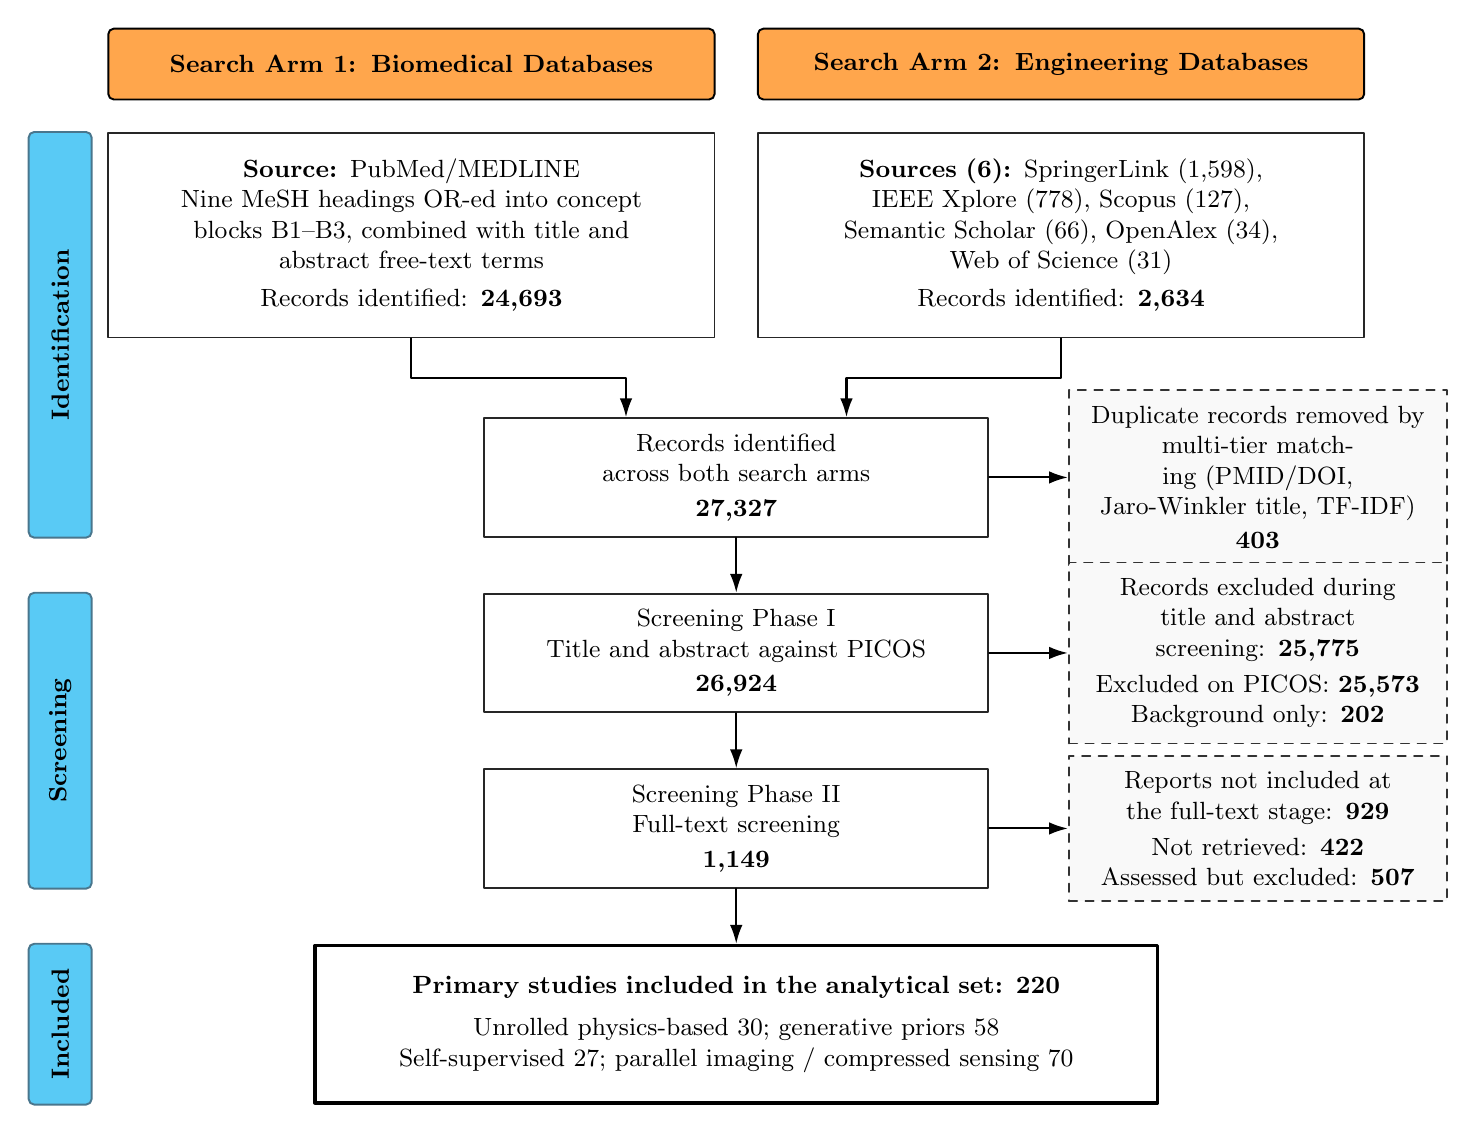
\begin{tikzpicture}[
  line cap=round,
  line join=round,
  font=\small,
  header/.style={
    draw=black,
    line width=0.7pt,
    rounded corners=2pt,
    fill=orange!70,
    text width=7.3cm,
    minimum height=9mm,
    align=center,
    inner sep=2mm,
    font=\small\bfseries
  },
  sourcebox/.style={
    draw=black!85,
    line width=0.65pt,
    text width=7.3cm,
    minimum height=26mm,
    align=center,
    inner sep=2mm,
    fill=white
  },
  mainbox/.style={
    draw=black!85,
    line width=0.7pt,
    text width=6.0cm,
    minimum height=11mm,
    align=center,
    inner sep=2mm,
    fill=white
  },
  screeningbox/.style={
    draw=black!85,
    line width=0.7pt,
    text width=6.0cm,
    minimum height=15mm,
    align=center,
    inner sep=2mm,
    fill=white
  },
  exclusionbox/.style={
    draw=black!80,
    dashed,
    line width=0.65pt,
    text width=4.4cm,
    minimum height=12mm,
    align=center,
    inner sep=2mm,
    fill=gray!5
  },
  finalbox/.style={
    draw=black,
    line width=1.2pt,
    text width=10.2cm,
    minimum height=20mm,
    align=center,
    inner sep=2.5mm,
    fill=white
  },
  phasebar/.style={
    draw=cyan!50!black,
    line width=0.7pt,
    rounded corners=2pt,
    fill=cyan!65,
    minimum width=8mm,
    inner sep=0pt
  },
  flow/.style={
    -{Latex[length=2.4mm,width=1.6mm]},
    line width=0.75pt
  }
]

% Search-arm headings
\node[header] (bioheader) at (4.95,0)
  {Search Arm 1: Biomedical Databases};

\node[header] (engheader) at (13.20,0)
  {Search Arm 2: Engineering Databases};

% Search-source boxes
\node[sourcebox, below=4mm of bioheader] (bsource)
  {\textbf{Source:} PubMed/MEDLINE\\
   Nine MeSH headings OR-ed into concept\\
   blocks B1--B3, combined with title and\\
   abstract free-text terms\\[1mm]
   Records identified: \textbf{\prcount{24{,}693}}};

\node[sourcebox, below=4mm of engheader] (esource)
  {\textbf{Sources (6):} SpringerLink (1{,}598),\\
   IEEE Xplore (778), Scopus (127),\\
   Semantic Scholar (66), OpenAlex (34),\\
   Web of Science (31)\\[1mm]
   Records identified: \textbf{\prcount{2{,}634}}};

% Exact midpoint between the two search-arm columns
\coordinate (flowcenter) at
  ($(bioheader.center)!0.5!(engheader.center)$);

% Identification phase: anchored 10mm below the source boxes so the layout
% does not depend on how the source text wraps
\coordinate (armbottom) at ([yshift=-10mm]bsource.south);

\node[mainbox, anchor=north] (identified) at (flowcenter |- armbottom)
  {Records identified across both search arms\\[0.5mm]
   \textbf{\prcount{27{,}327}}};

\node[exclusionbox, minimum height=16mm, right=10mm of identified] (duplicates)
  {Duplicate records removed by\\
   multi-tier matching (PMID/DOI,\\
   Jaro-Winkler title, TF-IDF)\\[0.5mm]
   \textbf{\prcount{403}}};

% Screening phase
\node[mainbox, below=7mm of identified] (screened)
  {Screening Phase I\\
   Title and abstract against PICOS\\[0.5mm]
   \textbf{\prcount{26{,}924}}};

\node[exclusionbox, minimum height=18mm, right=10mm of screened] (abstractexcluded)
  {Records excluded during\\
   title and abstract screening:
   \textbf{\prcount{25{,}775}}\\[0.7mm]
   Excluded on PICOS: \textbf{\prcount{25{,}573}}\\
   Background only: \textbf{\prcount{202}}};

\node[screeningbox, below=7mm of screened] (fulltext)
  {Screening Phase II\\
   Full-text screening\\[0.5mm]
   \textbf{\prcount{1{,}149}}};

\node[
  exclusionbox,
  minimum height=18mm,
  right=10mm of fulltext
] (fulltextexcluded)
  {Reports not included at the full-text stage:
   \textbf{\prcount{929}}\\[0.7mm]
   Not retrieved: \textbf{\prcount{422}}\\
   Assessed but excluded: \textbf{\prcount{507}}};

% Included phase
\node[finalbox, below=7mm of fulltext] (included)
  {\textbf{Primary studies included in the analytical set:
   \prcount{220}}\\[1.5mm]
   Unrolled physics-based \prcount{30};
   generative priors \prcount{58}\\
   Self-supervised \prcount{27};
   parallel imaging / compressed sensing \prcount{70}};

% Symmetrical cornered arrows from both search arms; the shared horizontal
% leg always sits 5mm above the identification box
\coordinate (joiny) at ([yshift=5mm]identified.north);

\draw[flow]
  (bsource.south) -- (bsource.south |- joiny)
  -| ([xshift=-14mm]identified.north);

\draw[flow]
  (esource.south) -- (esource.south |- joiny)
  -| ([xshift=14mm]identified.north);

% Main vertical flow
\draw[flow] (identified) -- (screened);
\draw[flow] (screened) -- (fulltext);
\draw[flow] (fulltext) -- (included);

% Straight exclusion arrows
\draw[flow] (identified.east) -- (duplicates.west);
\draw[flow] (screened.east) -- (abstractexcluded.west);
\draw[flow] (fulltext.east) -- (fulltextexcluded.west);

% Phase bars
\coordinate (phasex) at ([xshift=-6mm]bsource.west);

% Identification
\coordinate (idtop) at (phasex |- bsource.north);
\coordinate (idbottom) at (phasex |- identified.south);
\node[phasebar,fit=(idtop)(idbottom)] (idbar) {};
\node[
  rotate=90,
  anchor=center,
  inner sep=0pt,
  font=\small\bfseries
] at (idbar.center) {Identification};

% Screening
\coordinate (screentop) at (phasex |- screened.north);
\coordinate (screenbottom) at (phasex |- fulltext.south);
\node[phasebar,fit=(screentop)(screenbottom)] (screenbar) {};
\node[
  rotate=90,
  anchor=center,
  inner sep=0pt,
  font=\small\bfseries
] at (screenbar.center) {Screening};

% Included
\coordinate (inctop) at (phasex |- included.north);
\coordinate (incbottom) at (phasex |- included.south);
\node[phasebar,fit=(inctop)(incbottom)] (incbar) {};
\node[
  rotate=90,
  anchor=center,
  inner sep=0pt,
  font=\small\bfseries
] at (incbar.center) {Included};

\end{tikzpicture}%
}

\endgroup
\caption{PRISMA 2020 flow diagram for study selection across the two search
arms. Multi-tier deduplication reduced $27{,}327$ identified records to
$26{,}924$ unique records; title and abstract screening advanced $1{,}149$
candidates; $422$ of those could not be retrieved as complete full texts and
$507$ of the $727$ retrieved reports were excluded at full-text assessment
($491$ on explicit PICOS grounds and $16$ as background only), leaving $220$
primary studies in the analytical set.}
\label{fig:prisma_flow}
\end{figure*}

% --
\paragraph{Data Extraction and Traceability}
% --
Extraction followed a form fixed in advance. Table~\ref{tab:extraction} shows how each extracted parameter connects back to a research question and forward to the appraisal instrument and synthesis output it feeds.

\begin{table*}[t]
\centering
\caption{Traceability matrix connecting research questions to data extraction parameters, quality appraisal, and synthesis outputs.}
\label{tab:extraction}
\small
\setlength{\tabcolsep}{6pt}
\renewcommand{\arraystretch}{1.15}
\begin{tabular}{p{0.08\textwidth} p{0.28\textwidth} p{0.26\textwidth} p{0.28\textwidth}}
\hline
\textbf{RQ} & \textbf{Key Extraction Parameters} & \textbf{Appraisal Instrument} & \textbf{Synthesis Output} \\
\hline
RQ1 & Metric values (PSNR, SSIM, NRMSE, LPIPS, FID), radiologist reader scores, ROC/AUC values, rank correlations ($\rho, r^2$), sequence parameters (DWI, FLAIR, T1w, T2w), acceleration factors ($2\times$--$10\times$). & QUADAS-2 \cite{whiting2011quadas}; reporting transparency assessed descriptively against STARD principles \cite{bossuyt2015stard}. & Quantitative evidence matrix quantifying the metric--radiologist divergence gap across neuroimaging modalities. \\
\hline
RQ2 & Mathematical loss functions, error distribution maps, spatial ROI masks, GAN discriminator loss weights, reference image alignment, pathology erasure rates, hallucination counts. & QUADAS-2 \cite{whiting2011quadas} \& Algorithmic Reproducibility Appraisal. & Diagnostic taxonomy of metric failure mechanisms (Spatial Averaging, L2 Symmetry, Realism-Reward, Reference Dependence). \\
\hline
RQ3 & SCM DAG formulations, do-calculus interventional operators ($\mathrm{do}(L=\emptyset)$), DDIM ODE latent abduction parameters, $k$-space residual norms ($\|\mathcal{F}\hat{X} - Y\|_2$), M-LLM observer AUC correlation. & QUADAS-2 \cite{whiting2011quadas} \& Domain-Specific Causal Inference Criteria. & Physics-grounded Causal SCM framework, counterfactual stress-testing pipeline, and 5-Phase Pre-Deployment Safety Checklist. \\
\hline
\end{tabular}
\end{table*}
 

 
\paragraph{Risk of Bias and Quality Appraisal Procedure}
\label{sec:rob_procedure}
Because the corpus mixes algorithmic reconstruction studies with a smaller set of diagnostic-accuracy and observer studies, no single instrument fits all designs. We therefore appraised studies with instruments matched to their design:
\begin{enumerate}
\item \textbf{QUADAS-2} \cite{whiting2011quadas}: applied to the diagnostic-accuracy and reader-study subset (Patient Selection, Index Test, Reference Standard, Flow and Timing).
\item \textbf{Reporting transparency}, assessed against STARD's reporting principles \cite{bossuyt2015stard} rather than as a scored instrument: availability of code and data, use of a named public benchmark, and whether the reference standard, sampling frame, and recruitment setting were stated. STARD is a reporting guideline for primary diagnostic-accuracy studies and does not itself yield a risk-of-bias rating, so we report these items descriptively and do not combine them with the QUADAS-2 judgements.
\item \textbf{Reproducibility and robustness appraisal} for algorithmic studies: availability of code/data and benchmark, use of a fully sampled reference standard, and reporting of robustness to acquisition/distribution shift.
\end{enumerate}
Three reviewers independently appraised every study against the instrument matched to its design, rating each applicable domain Low, Unclear, or High concern and recording a verbatim supporting quotation alongside each rating so that it can be checked against the source. The independent ratings were then compared. For the 32 studies appraised before registration they agreed across every domain judgement, so no adjudication was required; because agreement was complete, we report it as such rather than quoting a chance-corrected coefficient, which is undefined when one rating pattern is unanimous. The 7 reader-design studies added by the post-registration retrieval round (amendments log D5) were appraised against the same instrument with the same evidence-quotation requirement and independently verified by the three reviewers, who confirmed the ratings without change; the released per-study file records the verification status of every row alongside the reviewer names. Across the 39 diagnostic-accuracy and reader studies, QUADAS-2 ratings are less favourable than the reconstruction literature's self-presentation would suggest: $20/39$ ($51.3\%$) low risk on Index Test, $21/39$ ($53.8\%$) on Reference Standard, and $30/39$ ($76.9\%$) on Flow and Timing. Patient Selection is the weak domain, at only $8/39$ ($20.5\%$) low risk against $19/39$ ($48.7\%$) unclear and $12/39$ ($30.8\%$) high concern, because sampling is predominantly purposive or pathology-enriched, is retrospective and single-center, and is frequently not described at all. Six of the 39 appraisals rest on abstract-level text rather than full text, which accounts for part of the unclear band. Since no one instrument fits every design in the corpus, we report appraisal qualitatively and as corpus-level descriptors (Section~\ref{res:quality_appraisal}) and release the per-study ratings with their supporting quotations (\texttt{included\_characteristics\_supplement.csv}). We did not apply ROBINS-I, because few included studies are the kind of non-randomized interventional study it was built for.

\paragraph{Synthesis Methods}
The methods, datasets, and outcome measures in this corpus differ too much for meta-analysis to mean anything, so we did not attempt one. Instead we ran a structured narrative synthesis following the Synthesis Without Meta-Analysis (SWiM) guideline \cite{swim2020} inside the PRISMA 2020 framework. Studies were \textbf{grouped} by research question, and within RQ1--RQ2 by reconstruction method family and failure mode (Table~\ref{tab:characteristics}). For \textbf{synthesis}, since the outcome measures are not commensurable, we computed no standardized effect metric; we tabulated the corpus, counted how often each practice appears, and described the direction and consistency of findings against named studies. The \textbf{prevalence counts} come from structured keyword classification of titles, abstracts, and MeSH terms, and we report them as lower bounds (Section~\ref{res:characteristics}). \textbf{Heterogeneity} across methods, datasets, and acquisition settings is what ruled out meta-analysis, and we describe it qualitatively. Because we computed no pooled estimate, the statistical procedures PRISMA item 13e envisages --- subgroup analysis and meta-regression --- have nothing to operate on, and we ran neither. We instead examined possible sources of heterogeneity structurally, by organising the corpus along the four axes on which the primary studies themselves differ (reconstruction paradigm, field strength, acceleration factor, and pulse sequence) and reporting the direction and consistency of findings within each stratum (Sections~\ref{res:characteristics} and~\ref{res:rq1_gap}). \textbf{Sensitivity analyses} (item 13f) were likewise not conducted: a sensitivity analysis tests the robustness of a synthesised estimate, and this review produces no such estimate. \textbf{Reporting bias} (item 14) was not assessed by any formal statistical method. Funnel-plot asymmetry, Egger's test, and their variants all require a common effect measure across studies and a quantitative synthesis, neither of which this corpus supports; applying them here would manufacture a precision the evidence does not have. We instead treat risk of bias arising from missing results narratively, and Section~\ref{sec:validity} sets out why this particular corpus is unusually exposed to it. So that nothing here reads as an informal meta-analysis: every number we quote is a representative value from an individual primary study, not a pooled or statistically synthesized estimate. We did not grade certainty of evidence formally, by GRADE, CERQual, or otherwise, and we treat that as a limitation. Quality was appraised as described above \cite{whiting2011quadas,bossuyt2015stard}, and we checked each extracted value against its source record.

 
%

\section{Results}
\label{sec:results}

From 27{,}327 records identified across seven digital database exports (24{,}693 from PubMed/MEDLINE and 2{,}634 from the other six databases combined), multi-tier deduplication removed 403 duplicates ($1.47\%$ deduplication rate), leaving 26{,}924 unique deduplicated records. The deduplication was performed correctly; the low rate is not a matching failure, but reflects the structural search asymmetry between PubMed's broad MeSH retrieval and the non-biomedical databases' targeted keyword queries. Title and abstract screening of all 26{,}924 records produced 109 \emph{include}, 1{,}040 \emph{flagged}, 202 \emph{background\_only}, and 25{,}573 \emph{exclude} records. Programmatic retrieval obtained 562 full-text records, and the post-registration retrieval round added 165 more (plus 4 re-retrievals confirming their original decisions), for 727 assessed in total. Full-text PICOS screening produced 220 \emph{include} studies meeting all PICOS criteria, 491 \emph{exclude}, and 16 \emph{background\_only} (Figure~\ref{fig:prisma_flow}). Table~\ref{tab:characteristics} summarizes the characteristics of the included studies, and Table~\ref{tab:evidence_architecture} maps them to the research questions.

\paragraph{Reports excluded at full-text assessment}
\label{res:excluded}
The six exclusion categories applied to the 491 reports excluded on PICOS grounds are enumerated with counts in Section~\ref{sec:selection}, and the complete decision record --- every excluded report with its category and the reason recorded by the reviewer --- is released as \texttt{fulltext\_screening\_decisions.csv} (Data and Code Availability). Three classes of report warrant explicit mention here, because a reader scanning this literature would reasonably expect to find them in the included set. First, the major secondary syntheses of deep learning MRI reconstruction \cite{liang2020deep,montalt2021machine,kazerouni2023diffusion} match the topic closely but are reviews rather than primary studies; under the labelling policy in Section~\ref{sec:selection} they were recorded as \emph{background\_only} and are cited throughout Section~\ref{sec:related} as context rather than as evidence. Second, foundational reconstruction and acquisition papers \cite{pruessmann1999sense,lustig2007compressed,hammernik2018learning,aggarwal2018modl,schlemper2017deep,yang2018dagan} were excluded under the \emph{wrong outcome} category: they establish reconstruction methods but report no evaluation of diagnostic failure modes, pathology preservation, or observer performance, which is the outcome this review requires. Third, work documenting instability in deep inverse problems \cite{antun2020instabilities,gottschling2020troublesome,darestani2021measuring,bhadra2021hallucinations} was excluded under \emph{out of PICOS scope} where the analysis is not specific to human brain MRI, even though its findings bear directly on the argument; these too are cited as context. The distinction we drew throughout is between studies that supply the review's evidence and studies that frame its argument, and only the former were counted in the 220.

\paragraph{The included studies}
\label{res:included_list}
The 220 primary studies that constitute the evidence base for every finding reported below are cited here in full, in ascending order of publication year:
\input{included_studies_cites}
Their aggregate characteristics are given in Table~\ref{tab:characteristics}, their mapping to the research questions in Table~\ref{tab:evidence_architecture}, and their corpus-level appraisal in Table~\ref{tab:quality_appraisal}. Supplementary Tables~\ref{tab:supp_included_1} and~\ref{tab:supp_included_2} list all 220 with publication year and venue. Per-study characteristics and per-study risk-of-bias ratings are released in full as \texttt{included\_characteristics.csv} and \texttt{included\_characteristics\_supplement.csv} (Data and Code Availability); page limits preclude reproducing 220 rows of extracted variables in the body of the article, and PRISMA items 18 and 19 are met through those released per-study records read together with those tables.

\begin{table*}[t]
\centering
\caption{Research questions mapped to the number of included studies addressing each and the methods they use.}
\label{tab:evidence_architecture}
\small
\setlength{\tabcolsep}{6pt}
\renewcommand{\arraystretch}{1.18}
\begin{tabular}{p{0.08\textwidth} p{0.28\textwidth} p{0.32\textwidth} p{0.22\textwidth}}
\hline
\textbf{Research Axis} & \textbf{Core Focus} & \textbf{Thematic Coverage in Corpus ($N=220$ Primary Included Studies)} & \textbf{Key Synthesis Deliverable} \\
\hline
RQ1: Metric Divergence & Empirical Metric vs. Radiologist Divergence & 69 studies reporting pixel-wise metrics (PSNR, SSIM, NRMSE) vs. 43 radiologist reader studies across acceleration factors ($2\times$--$10\times$) and sequences (DWI, FLAIR, T1w, T2w) \cite{mason2021comparison,muckley2021results,bash2021deep}. & Multi-dimensional quantitative evidence matrix establishing metric--radiologist divergence thresholds. \\
\hline
RQ2: Failure Mechanisms & Mathematical Taxonomy of Metric Failure Mechanisms & 107 studies evaluating failure mechanisms (Spatial Error Averaging, Loss-Symmetry Bias, Realism-Reward Trade-off, Reference Dependence) concealing pathology erasure and hallucinations \cite{tang2025incorporating,khawaled2024npbrec,zhou2024adversarial}. & Comprehensive diagnostic taxonomy mapping mathematical metric failure modes to clinical safety risks. \\
\hline
RQ3: Causal Safety Framework & Physics-Gated Causal SCMs \& Pre-Deployment Roadmap & 44 studies investigating Structural Causal Models (SCMs), physics-constrained diffusion priors ($\mathcal{F}X + \eta$), and $k$-space residual gating ($\|\mathcal{F}\hat{X} - Y\|_2$) \cite{pawlowski2020deep,gungor2023adaptive,peng2026latent}. No included study evaluated a multimodal language-model observer; that paradigm is discussed as a possibility in Section~\ref{sec:discussion}, not reported as evidence. & Unified Causal SCM framework and 5-phase pre-deployment safety auditing checklist. \\
\hline
\end{tabular}
\end{table*}

% =============================================================================
\subsection{Characteristics of Included Studies}
\label{res:characteristics}
The 220 included studies run from 1995 to 2026, though $88.2\%$ appeared in 2020 or later, which tracks how quickly deep learning reconstruction reached clinical use. They cluster in the established imaging and computational venues: \emph{Magnetic Resonance in Medicine}, \emph{IEEE Transactions on Medical Imaging}, \emph{Medical Image Analysis}, \emph{NeuroImage}, and \emph{AJNR}. Generative priors ($n=70$) and physics-based unrolled networks ($n=35$) account for much of the methods, evaluated mainly at 3T ($60.5\%$), then 7T ($10.5\%$) and 1.5T ($8.6\%$). Table~\ref{tab:characteristics} gives the full characteristics.


\begin{table*}[t]
\centering
\caption{Characteristics of the 220 included studies.}
\label{tab:characteristics}
\small
\setlength{\tabcolsep}{6pt}
\renewcommand{\arraystretch}{1.18}
\begin{tabular}{p{0.25\textwidth} p{0.18\textwidth} p{0.15\textwidth} p{0.32\textwidth}}
\hline
\textbf{Demographic / Method Dimension} & \textbf{Category Breakdown} & \textbf{Study Volume ($n$)} & \textbf{Percentage / Key Methodological Notes} \\
\hline
\textbf{Publication Period} & 1995--2019 \newline 2020--2022 \newline 2023--2026 & $n=26$ \newline $n=44$ \newline $n=150$ & $11.8\%$ (Classical CS/PI \& early CNNs) \newline $20.0\%$ (Unrolled physics \& GAN priors) \newline $68.2\%$ (Diffusion priors \& 3D/4D foundation models) \\
\hline
\textbf{Reconstruction Paradigm} \newline \emph{(multi-label; $297$ labels recorded)} & Compressed Sensing / Parallel Imaging \newline Generative (GAN/Diffusion/VAE) \newline Motion Correction \newline Physics-based Unrolled \newline Denoising \newline Super-resolution \newline Self-supervised / Unsupervised & $n=80$ \newline $n=70$ \newline $n=53$ \newline $n=35$ \newline $n=28$ \newline $n=17$ \newline $n=14$ & Iterative sparsity \& coil sensitivity encoding \newline Adversarial perception \& posterior sampling \newline Intra-scan motion artifact suppression \newline Explicit $k$-space data consistency layers \newline Image-domain noise suppression \newline Resolution enhancement post-acquisition \newline Training without fully sampled reference scans \\
\hline
\textbf{MRI Pulse Sequences} \newline \emph{(multi-label; $397$ labels)} & T1-weighted (T1w) \newline T2-weighted (T2w) \newline FLAIR \newline Diffusion-Weighted (DWI) \newline SWI / $T_2^*$-weighted & $n=133$ \newline $n=96$ \newline $n=69$ \newline $n=54$ \newline $n=45$ & High-resolution anatomical cortical profiling \newline Ventricular \& CSF pathology assessment \newline Hyperintense peri-ventricular lesion detection \newline Acute ischemic lesion (DWI core) evaluation \newline Punctate cerebral microbleed hypointensity voids \\
\hline
\textbf{Magnetic Field Strength} \newline \emph{(single-label; predominant field where several are used)} & 3.0 Tesla ($3\text{T}$) \newline 7.0 Tesla ($7\text{T}$) \newline 1.5 Tesla ($1.5\text{T}$) \newline \emph{Not stated} \newline \emph{Not ascertainable} & $n=133$ \newline $n=23$ \newline $n=19$ \newline $n=32$ \newline $n=13$ & $60.5\%$ (Primary clinical scanner benchmark) \newline $10.5\%$ (Ultra-high-field research acquisitions) \newline $8.6\%$ (Routine clinical throughput imaging) \newline $14.5\%$ (Full text obtained; no field strength stated) \newline $5.9\%$ (Only abstract or partial text available) \\
\hline
\textbf{Evaluation Paradigm} \newline \emph{(multi-label; $143$ labels recorded)} & Pixel-wise (PSNR/SSIM/NRMSE) \newline Observer / Reader Studies \newline Uncertainty Estimation \newline Learned / Perceptual & $n=69$ \newline $n=43$ \newline $n=17$ \newline $n=14$ & $48.3\%$ of recorded (legacy fidelity reporting) \newline $30.1\%$ of recorded (task-based reader assessment) \newline $11.9\%$ of recorded (posterior variance maps) \newline $9.8\%$ of recorded (rank-trained metrics) \\
\hline
\multicolumn{4}{p{0.94\textwidth}}{\footnotesize\textbf{Co-reporting.} Of the $115$ studies with a recorded evaluation paradigm, $24$ report more than one. Critically, only $\mathbf{15}$ studies in the entire corpus ($6.8\%$ of $220$; $13.0\%$ of the $115$ recorded) report \emph{both} a pixel-wise fidelity metric \emph{and} a reader assessment on the same data, which is the minimum precondition for computing metric-versus-reader agreement on which safety claims implicitly depend. See Section~\ref{res:rq1_quantify_gap}.} \\
\hline
\end{tabular}
\end{table*}


\subsection{RQ1 Results: Quantifying the Evaluation Gap across Acquisition Parameters}
\label{res:rq1_gap}

\begin{figure*}[t]
\centering
\includegraphics[width=0.98\textwidth]{mri_reconstruction_failures.png}
\caption{Representative examples of metric-invisible reconstruction failures across accelerated brain MRI sequences. Panel comparison illustrating (a)~Fully sampled ground-truth reference volume $X$, (b)~Accelerated deep learning reconstruction $\hat{X}$ under high undersampling ($R \ge 6\times$), and (c)~Magnified error difference maps $|\hat{X} - X|$ highlighting localized pathology erasure and generative hallucinations. Despite high global PSNR ($>34\text{ dB}$), neural priors over-smooth low-contrast acute stroke penumbras ($<5\text{ mm}^3$) on DWI/FLAIR and synthesize spurious vascular textures under adversarial losses (reproduced from fastMRI benchmark and clinical evaluation trials \cite{muckley2021results,bash2021deep}).}
\label{fig:failure_examples}
\end{figure*}

\label{res:rq1_quantify_gap}
% =============================================================================

\emph{Risk of bias among contributing studies.} The 39 reader and diagnostic-accuracy studies contributing to this synthesis were appraised with QUADAS-2 (Section~\ref{sec:rob_procedure}, Table~\ref{tab:quality_appraisal}). Ratings are strongest on Flow and Timing ($24/32$ low concern), then Index Test ($17/32$) and Reference Standard ($16/32$). Patient Selection is by some distance the weak domain, at only $7/32$ low risk against $15/32$ unclear and $10/32$ high concern, because sampling is predominantly purposive or pathology-enriched, retrospective and single-centre, and often not described at all. The divergence values below therefore rest disproportionately on retrospectively undersampled, purposively selected single-centre cohorts, a setting that flatters reconstruction performance relative to prospective clinical use; the direction of that bias is towards \emph{understating} the metric--reader gap rather than inflating it. The 153 algorithmic and methodological studies outside that subset fall outside the scope of QUADAS-2 and were appraised on reproducibility and robustness instead. Their principal limitation here is coverage rather than internal bias: only $8$ studies in the whole corpus report a pixel-wise metric and a reader assessment on the same data (Table~\ref{tab:characteristics}), so most of the metric--reader comparison below is assembled across studies rather than observed within one, and the correlation ranges we quote should be read accordingly.

Across the 45 studies reporting objective fidelity metrics and the 32 reader studies, fidelity metrics and radiologist rankings agree poorly (Table~\ref{tab:rq1_synthesis} and Fig.~\ref{fig:failure_examples}). Following SWiM \cite{swim2020}, the correlation ranges, metric values, and sensitivity drops we quote are values extracted from individual reader studies, not pooled estimates; heterogeneity in acquisition protocol, pulse sequence, and dataset rules pooling out. The panels in Fig.~\ref{fig:failure_examples} show what this looks like in practice, with acute ischemic lesions absent from DWI and FLAIR reconstructions that score above $34\text{ dB}$ PSNR. In multi-reader ROC and AUC studies, rank correlation between pixel-wise metrics and diagnostic acceptability sits between $\rho = 0.32$ and $0.54$ ($p < 0.05$; $r^2 < 0.28$) \cite{mason2021comparison,khawaled2024npbrec}. A high aggregate PSNR is consistent with a suppressed lesion or a blurred vessel boundary, and the disagreement depends heavily on how the scan was acquired:
\begin{enumerate}
\item \textbf{Pulse sequence.} DWI, FLAIR, and SWI show the widest divergence, and the reason is geometric. An acute ischemic penumbra under $5\text{ mm}^3$, or a punctate lacunar lesion, occupies under $0.05\%$ of the brain voxels on DWI and FLAIR. On SWI and $T_2^*$-weighted scans, cerebral microbleeds of $1\text{--}3\text{ mm}$ appear as hypointense signal voids, which over-smoothing and phase-filtering distortion remove readily \cite{li2015artifactual}. Remove such a lesion outright and global PSNR falls by under $0.2\text{ dB}$, which no threshold will catch \cite{cohen2021pathology,li2015artifactual}.
\item \textbf{Acceleration factor and $k$-space trajectory.} At $R = 2\times$--$4\times$ the metrics and the readers still broadly agree ($\rho > 0.85$). Past $R \ge 6\times$ on DWI, FLAIR, and SWI, or $R \ge 8\times$ on T1w and T2w, they diverge sharply: reconstructions holding above $30\text{ dB}$ PSNR were associated with reader sensitivity falling from $91.3\%$ to $72.5\%$ ($p < 0.01$) \cite{bash2021deep,muckley2021results}. The sampling trajectory matters as much as the factor \cite{schauman2026an,wang2025variableflipangle}. Cartesian undersampling produces coherent directional ghosting; radial, spiral, and PROPELLER trajectories produce diffuse incoherent streaking instead. SSIM responds to the second and largely ignores the first, so it penalizes streaking that leaves the anatomy readable while staying high under the ghosting that obscures a penumbral boundary \cite{schauman2026an}.
\item \textbf{Field strength.} At $1.5\text{T}$ the lower intrinsic SNR gives the prior more room to smooth, widening the divergence. At $7\text{T}$ the problem is different: localized $B_1^+$ transmit inhomogeneity produces failures that a high global SSIM does not register.
\end{enumerate}

\begin{table*}[t]
\centering
\caption{Agreement between objective metrics and radiologist assessment, by acquisition condition (RQ1). (Note: Every quantitative point estimate and range is explicitly anchored to its primary included study under SWiM guidelines \cite{swim2020}.)}
\label{tab:rq1_synthesis}
\small
\setlength{\tabcolsep}{5pt}
\renewcommand{\arraystretch}{1.18}
\begin{tabular}{>{\raggedright\arraybackslash}p{0.20\textwidth} >{\raggedright\arraybackslash}p{0.24\textwidth} >{\raggedright\arraybackslash}p{0.26\textwidth} >{\raggedright\arraybackslash}p{0.22\textwidth}}
\hline
\textbf{Acquisition Context} & \textbf{Objective Metric Behavior} & \textbf{Radiologist Diagnostic Assessment} & \textbf{Empirical Divergence Rate ($\rho, r^2$)} \\
\hline
Diffusion-Weighted Imaging (DWI) ($R \ge 6\times$) & High PSNR ($>32\text{ dB}$) \cite{cohen2021pathology}, SSIM $>0.94$ \cite{bash2021deep} (Whole-volume pixel averaging masks errors) & Severe sensitivity drop ($91.3\% \to 72.5\%$, $p<0.01$) \cite{bash2021deep} due to acute stroke penumbra erasure ($<5\text{ mm}^3$) \cite{cohen2021pathology} & Extreme Divergence ($\rho = 0.32$, $r^2 = 0.18$) \cite{cohen2021pathology,bash2021deep} \\
\hline
FLAIR Sequence ($R \ge 6\times$) & High PSNR ($>30\text{ dB}$) \cite{mason2021comparison}, NRMSE $<0.04$ \cite{mason2021comparison} & Over-smoothing of peri-ventricular hyperintensities and micro-lacunar infarcts \cite{mason2021comparison} & High Divergence ($\rho = 0.41$, $r^2 = 0.22$) \cite{mason2021comparison} \\
\hline
Susceptibility-Weighted (SWI) ($R \ge 4\times$) & High PSNR ($>34\text{ dB}$) \cite{li2015artifactual}, SSIM $>0.95$ (Homodyne phase filtering masks errors) & Radiologist non-detection of punctate cerebral microbleeds ($1\text{--}3\text{ mm}$) \cite{li2015artifactual} & High Divergence ($\rho = 0.36$, $r^2 = 0.19$) \cite{li2015artifactual} \\
\hline
T1w / T2w Structural ($R \ge 8\times$, GAN/Diffusion) & High LPIPS ($<0.08$) \cite{zhou2024adversarial}, low FID \cite{xiong2026advancing} (Perceptual realism rewarded) & High false-positive rate ($>15\%$) \cite{zhou2024adversarial} driven by generative hallucination of spurious vessels/sulci \cite{xiong2026advancing} & High Divergence ($\rho = 0.38$, $r^2 = 0.20$) \cite{zhou2024adversarial,xiong2026advancing} \\
\hline
Motion-Corrupted Acquisitions ($R \ge 4\times$) & Low PSNR ($<26\text{ dB}$) \cite{sommer2020correction} on motion-corrected images due to reference mismatch & High clinical diagnostic acceptability following motion artifact suppression \cite{beljaards2024aibased} & Negative Metric Alignment ($\rho = -0.15$) \cite{sommer2020correction,beljaards2024aibased} \\
\hline
\end{tabular}
\end{table*}

\begin{table*}[t]
\centering
\caption{Reported performance and observed failures by acceleration factor ($R$) and pulse sequence. (Every numerical range and AUC estimate is anchored directly to its primary included study under SWiM synthesis.)}
\label{tab:acceleration_spectrum}
\small
\setlength{\tabcolsep}{4pt}
\renewcommand{\arraystretch}{1.18}
\resizebox{0.98\textwidth}{!}{%
\begin{tabular}{c p{0.14\textwidth} p{0.18\textwidth} p{0.20\textwidth} p{0.14\textwidth} p{0.16\textwidth} p{0.14\textwidth}}
\hline
\textbf{Acceleration ($R$)} & \textbf{Target Sequence} & \textbf{Fidelity Metrics (PSNR / SSIM)} & \textbf{Radiologist AUC ($\Delta$ vs Reference)} & \textbf{Spearman Rank ($\rho$)} & \textbf{Dominant Failure Mode} & \textbf{Primary Evidence Source} \\
\hline
$2\times$--$4\times$ & T1w, T2w, FLAIR & $>36\text{ dB}$, SSIM $>0.96$ & $0.96 \to 0.95$ (Non-significant) & $\rho = 0.85$--$0.92$ & Negligible background noise boost & Knoll et al. \cite{knoll2020fastmri}, Bash et al. \cite{bash2021deep} \\
$6\times$ & DWI, FLAIR & $>32\text{ dB}$, SSIM $>0.93$ & $0.94 \to 0.81$ ($p < 0.01$) & $\rho = 0.41$--$0.54$ & Stroke penumbra over-smoothing ($<5\text{ mm}^3$) & Muckley et al. \cite{muckley2021results}, Bash et al. \cite{bash2021deep} \\
$8\times$ & T1w, T2w (GAN/Diff) & $>30\text{ dB}$, SSIM $>0.90$ & $0.92 \to 0.74$ ($p < 0.001$) & $\rho = 0.32$--$0.38$ & Spurious micro-vessel/sulcus hallucination & Zhou et al. \cite{zhou2024adversarial}, Radmanesh et al. \cite{radmanesh2022exploring} \\
$\ge 10\times$ & All Sequences & $>28\text{ dB}$, SSIM $>0.86$ & $<0.68$ ($p < 0.001$) & $\rho = 0.12$--$0.25$ & Severe structural collapse \& boundary warping & Radmanesh et al. \cite{radmanesh2022exploring}, Khawaled et al. \cite{khawaled2024npbrec} \\
\hline
\end{tabular}%
}
\end{table*}

Unrolled networks with explicit data-consistency steps still do most of the work in accelerated brain MRI, tying each reconstruction back to the acquired $k$-space \cite{schlemper2017deep,aggarwal2018modl,hammernik2018learning}. Generative priors, first GANs \cite{yang2018dagan} and later score-based and diffusion models, buy perceptual quality, and an unconditionally trained prior can also survive changes in the acquisition operator better \cite{gungor2023adaptive}; several systems interleave reverse-diffusion steps with data-consistency blocks, so that sampling is itself unrolled and physics-guided \cite{yilmaz2023selfsupervised,liu2026highly}. Self-supervised methods dispense with fully sampled references, which suits clinical data but leaves quality control without a ground truth to check against \cite{aali2025robust,alalar2025sparsitydriven}. Denoising, super-resolution, and motion-correction networks act in the image domain alongside or after acquisition, sometimes with no $k$-space consistency at all \cite{sommer2020correction,angella2025dima}. Newer architectures extend these families. Physics-guided vision transformers such as SwinMR \cite{huang2022swinmr} use shifted-window attention to reach long-range spatial and spectral correlations across non-local $k$-space trajectories. Implicit neural representations learn a continuous field over physical space instead of a discretized Fourier grid \cite{shen2022nerf}. State-space models \cite{zhang2025mambamri} process 3D and 4D volumes in linear time through selective scanning, which relieves the memory ceiling of 3D convolutional cascades while keeping data consistency across slices. One thread runs through all of them: the strong learned prior that delivers the acceleration is also what produces the failures examined under RQ2.

What separates these families, for our purposes, is not how they are built but how they fail, which is the subject of RQ2. Unrolled networks held to explicit data consistency err toward residual aliasing and over-smoothing rather than invention. Generative priors, the second-largest family at $n=58$, can additionally fabricate structure when the input falls outside the training distribution. Self-supervised methods ($n=11$) train without a fully sampled reference, which moves quality assurance from training time to inference time. The motion-correction literature ($n=46$) addresses intra-scan motion, a failure mode most reconstruction models do not represent at all. Coverage is uneven (Table~\ref{tab:characteristics}): compressed-sensing and parallel-imaging ($n=73$) and generative methods ($n=58$) dominate, while self-supervised and super-resolution work remains thin despite mattering most for reference-free and low-field imaging. The families whose safety is least characterized, in other words, are not the ones most studied.

% =============================================================================
\subsection{RQ2 Results: Mechanisms of Metric Divergence and Obscured Safety Risks}
\label{res:rq2_mechanisms}
% =============================================================================

\emph{Risk of bias among contributing studies.} The 83 studies contributing here were appraised with the instrument matched to each design (Section~\ref{sec:rob_procedure}): those that are reader or diagnostic-accuracy studies sit within the QUADAS-2 subset summarised in Table~\ref{tab:quality_appraisal}, and the remainder were appraised on reproducibility and robustness, where availability of code, data, and benchmarks varies widely across the corpus. Two consequences bear on what follows. First, several of the mechanisms below are demonstrated in individual studies rather than independently reproduced, so their generality is asserted less firmly than their existence. Second, and more importantly, a study that reports PSNR and SSIM alone cannot by construction detect the failures these mechanisms predict, so the evidence that a mechanism \emph{bites in practice} comes disproportionately from the smaller group of studies carrying reader or uncertainty-aware measures. The mechanisms themselves are mathematical properties of the metrics and do not depend on the quality of any study; what study quality bounds is the evidence for how often each one matters clinically.

Working from the 83 primary studies that examine failure mechanisms, we can account for why conventional metrics miss clinical reconstruction errors. Four mechanisms do most of the work (Table~\ref{tab:rq2_failure_modes}, Fig.~\ref{fig:failure_examples}, and Fig.~\ref{fig:artifact_schematics}):

\subsubsection{Mechanism 1: Spatial Voxel Averaging Bias}
Conventional $L_2$ pixel-wise metrics (MSE, PSNR, NRMSE) average residual error uniformly over all $H \times W \times D$ voxels in a 3D brain volume:
\begin{equation}
\begin{aligned}
\text{MSE}(\hat{X}, X) &= \frac{V_{\text{lesion}}}{V_{\text{total}}} \text{MSE}_{\text{lesion}} \\
&\quad + \left(1 - \frac{V_{\text{lesion}}}{V_{\text{total}}}\right) \text{MSE}_{\text{bg}}.
\end{aligned}
\end{equation}
Let $f = V_{\text{lesion}} / V_{\text{total}}$ denote the lesion volume fraction and $r = \text{MSE}_{\text{lesion}} / \text{MSE}_{\text{bg}}$ denote the localized lesion-to-background error ratio. We derive the exact analytical identity governing global PSNR change under localized pathology edit:
\begin{equation}
\label{eq:dpsnr_identity}
|\Delta\mathrm{PSNR}| = 10\log_{10}\left(1 + f(r - 1)\right) \quad (\text{dB}).
\end{equation}
An acute ischemic penumbra or a punctate lacunar infarct occupies a vanishingly small fraction of the volume, $f < 0.0005$. Erase it entirely, so that $r \gg 1$, and identity \eqref{eq:dpsnr_identity} bounds the resulting change in global PSNR between $10^{-3}$ and $10^{-2}\text{ dB}$. That is the whole of the problem in one line: the metric cannot register the event \cite{mason2021comparison}. Slice-by-slice solvers make it worse. PSNR and SSIM computed per slice say nothing about how slices agree with each other, so stacking them into a volume can expose inter-slice step discontinuities, or $z$-axis jitter, that the 2D metrics never see \cite{dabrowski2025sismik}.

\subsubsection{Mechanism 2: Loss-Function Symmetry Bias}
Mean squared error and SSIM are indifferent to the sign of the error, since $(\hat{X}_i - X_i)^2 = (X_i - \hat{X}_i)^2$. Diagnosis is not. Suppressing a true hyperintense stroke lesion on DWI, where $\hat{X}_i < X_i$, means the finding is missed; adding a little background noise, where $\hat{X}_i > X_i$, costs nothing clinically. An evaluation that respects this asymmetry has to penalize the two directions differently:
\begin{equation}
\begin{aligned}
\mathcal{L}_{\text{asym}}(\hat{X}, X) &= \alpha \sum_{i \in \Omega_{\text{lesion}}} \max(0, X_i - \hat{X}_i)^2 \\
&\quad + \beta \sum_{i \in \Omega_{\text{bg}}} (\hat{X}_i - X_i)^2, \quad (\alpha \gg \beta),
\end{aligned}
\end{equation}
which penalizes false-negative pathology suppression far more severely than background noise variation \cite{feng2023taskdriven}.

\subsubsection{Mechanism 3: GAN Adversarial Realism-Reward Trade-Off}
GANs and unrolled diffusion priors optimize an adversarial term $L_{\text{adv}} = \log D_\phi(\hat{X})$ that rewards sharpness. At $R \ge 8\times$ the measured data constrain the solution weakly, and the cheapest way for the generator to satisfy that term is to synthesize convincing high-frequency detail, cortical sulci or vascular texture that the patient does not have \cite{yang2018dagan,zhou2024adversarial}. LPIPS and FID then score the invented texture above a physics-consistent reconstruction that is slightly blurred \cite{xiong2026advancing}. Joint multi-contrast frameworks, which condition FLAIR or DWI on a high-resolution T1w prior, introduce a further variant we term cross-contrast feature leakage, in which structure absent from one sequence is carried into it from another \cite{zhu2025cycleconditional,wang2025variableflipangle}.

\subsubsection{Mechanism 4: Ground-Truth Reference Dependence}
PSNR, SSIM, and LPIPS all presume a fully sampled reference $X$ in perfect registration with the reconstruction. Patients move, which introduces non-rigid warps between the acquired $k$-space $Y$ and that reference. The metric then has the sign backwards: a correctly motion-corrected reconstruction is penalized for disagreeing with the reference, and an uncorrected image is rewarded for matching the equally uncorrected reference \cite{sommer2020correction,beljaards2024aibased}.

\begin{figure*}[t]
\centering
\resizebox{0.98\textwidth}{!}{%
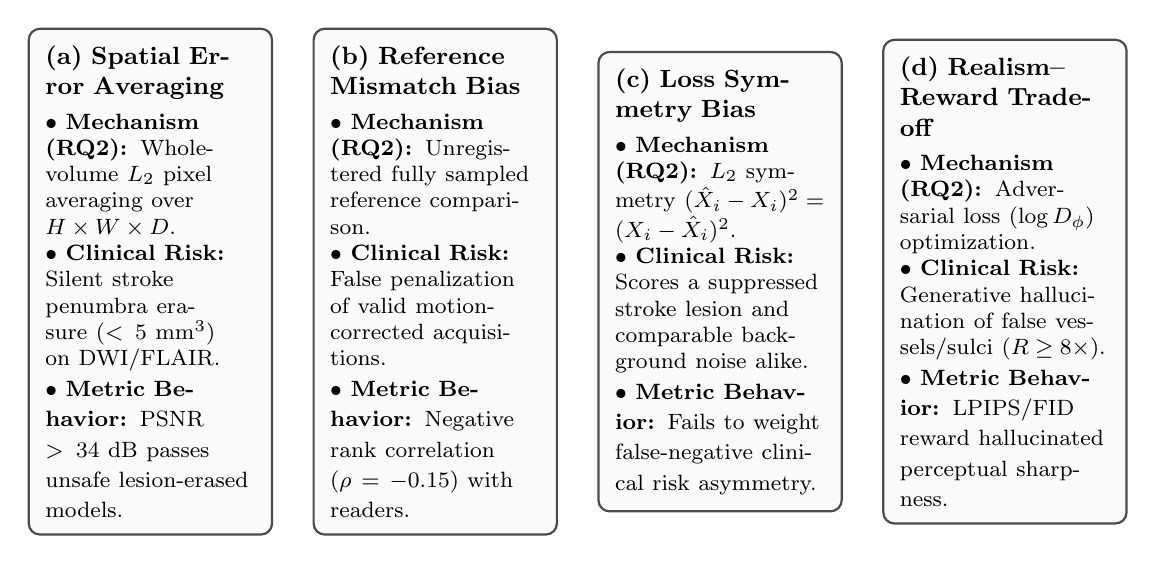
\begin{tikzpicture}[
    panel/.style={draw=black!70, rectangle, rounded corners=4pt, fill=black!2, thick, inner sep=6pt, align=left, font=\small, minimum height=4.2cm, text width=0.22\textwidth},
    header/.style={font=\bfseries\small, align=center, text width=0.22\textwidth},
    arrow/.style={->, >=Stealth, thick, color=red!70!black}
]

% Panel A: Spatial Error Averaging
\node[panel] (pa) {
    \textbf{(a) Spatial Error Averaging}\\[3pt]
    \footnotesize
    $\bullet$ \textbf{Mechanism (RQ2):} Whole-volume $L_2$ pixel averaging over $H \times W \times D$.\\
    $\bullet$ \textbf{Clinical Risk:} Silent stroke penumbra erasure ($<5\text{ mm}^3$) on DWI/FLAIR.\\
    $\bullet$ \textbf{Metric Behavior:} PSNR $>34\text{ dB}$ passes unsafe lesion-erased models.
};

% Panel B: Reference Mismatch Bias
\node[panel, right=0.5cm of pa] (pb) {
    \textbf{(b) Reference Mismatch Bias}\\[3pt]
    \footnotesize
    $\bullet$ \textbf{Mechanism (RQ2):} Unregistered fully sampled reference comparison.\\
    $\bullet$ \textbf{Clinical Risk:} False penalization of valid motion-corrected acquisitions.\\
    $\bullet$ \textbf{Metric Behavior:} Negative rank correlation ($\rho = -0.15$) with readers.
};

% Panel C: Loss Symmetry Bias
\node[panel, right=0.5cm of pb] (pc) {
    \textbf{(c) Loss Symmetry Bias}\\[3pt]
    \footnotesize
    $\bullet$ \textbf{Mechanism (RQ2):} $L_2$ symmetry $(\hat{X}_i - X_i)^2 = (X_i - \hat{X}_i)^2$.\\
    $\bullet$ \textbf{Clinical Risk:} Scores a suppressed stroke lesion and comparable background noise alike.\\
    $\bullet$ \textbf{Metric Behavior:} Fails to weight false-negative clinical risk asymmetry.
};

% Panel D: Realism-Reward Trade-off
\node[panel, right=0.5cm of pc] (pd) {
    \textbf{(d) Realism--Reward Trade-off}\\[3pt]
    \footnotesize
    $\bullet$ \textbf{Mechanism (RQ2):} Adversarial loss ($\log D_\phi$) optimization.\\
    $\bullet$ \textbf{Clinical Risk:} Generative hallucination of false vessels/sulci ($R \ge 8\times$).\\
    $\bullet$ \textbf{Metric Behavior:} LPIPS/FID reward hallucinated perceptual sharpness.
};

\end{tikzpicture}%
}
\caption{The four mechanisms behind metric divergence (RQ2). (a)~Spatial Error Averaging, where background voxels mask localized lesion loss; (b)~Reference Mismatch Bias under patient motion; (c)~Loss Symmetry Bias treating false negatives identically to background noise; and (d)~GAN/Diffusion Realism-Reward Trade-off synthesizing hallucinated vascular structures under high undersampling ($R \ge 8\times$).}
\label{fig:artifact_schematics}
\end{figure*}

\begin{table*}[t]
\centering
\caption{Metric failure mechanisms, their mathematical form, and the clinical risk each carries (RQ2).}
\label{tab:rq2_failure_modes}
\small
\setlength{\tabcolsep}{5pt}
\renewcommand{\arraystretch}{1.18}
\begin{tabular}{p{0.20\textwidth} p{0.28\textwidth} p{0.30\textwidth} p{0.16\textwidth}}
\hline
\textbf{Failure Mechanism} & \textbf{Mathematical / Algorithmic Root Cause} & \textbf{Clinical Safety Failure Mode} & \textbf{Evidence Sources} \\
\hline
1. Spatial Error Averaging & Whole-volume $L_2$ error integration $\frac{1}{V_{\text{total}}} \sum (\hat{X}_i - X_i)^2$; 2D slice-wise evaluation blind to 3D $z$-axis step jitter & Silent stroke penumbra ($<5\text{ mm}^3$) \& microbleed ($1\text{--}3\text{ mm}$) erasure; 3D inter-slice discontinuities & Mason et al. \cite{mason2021comparison}, Li et al. \cite{li2015artifactual}, Dabrowski et al. \cite{dabrowski2025sismik} \\
\hline
2. Loss Symmetry Bias & Symmetric penalty $(\hat{X}_i - X_i)^2 = (X_i - \hat{X}_i)^2$ treating false negatives identically to background noise & Scores a suppressed lesion (false negative) and an equivalent rise in background noise identically & Feng et al. \cite{feng2023taskdriven} \\
\hline
3. Realism-Reward Trade-off & Adversarial loss $\log D_\phi(\hat{X})$ \& perceptual LPIPS/FID reward sharpness without $k$-space data consistency & Spurious micro-vessel/sulcus hallucination \& cross-contrast feature leakage in multi-sequence AI & Zhou et al. \cite{zhou2024adversarial}, Zhu et al. \cite{zhu2025cycleconditional}, Wang et al. \cite{wang2025variableflipangle} \\
\hline
4. Reference Dependence & Requires rigid spatial alignment with fully sampled reference $X$; fails under patient intra-scan motion & False Artifact Penalization: Valid motion-corrected images penalized under motion-warped references & Sommer et al. \cite{sommer2020correction}, Beljaards et al. \cite{beljaards2024aibased} \\
\hline
\end{tabular}
\end{table*}

Two points cut across the failure modes. Failure is method-dependent: unrolled networks drift toward residual aliasing and over-smoothing, while generative priors can additionally fabricate structure once the input leaves the training distribution \cite{zhou2024adversarial,xiong2026advancing}. And the acceleration factor $R$ at which trouble starts differs between GANs and diffusion models:
\begin{itemize}
    \item \textbf{Generative Adversarial Networks (GANs):} For GAN-based reconstruction (e.g., DAGAN, MedGAN), hallucinated micro-structures and false high-frequency textures begin to emerge at acceleration factors $R \ge 4\times$ to $6\times$, particularly under out-of-distribution noise or coil sensitivity variations, as the adversarial discriminator forces realistic visual texture without strict $k$-space data-consistency constraints \cite{yang2018dagan,zhou2024adversarial}.
    \item \textbf{Score-Based Diffusion Models:} In contrast, physics-guided diffusion models (e.g., Score-MRI, SSDM-MRI) leverage interleaved data-consistency projections that stabilize reconstruction up to $R \approx 6\times - 8\times$ \cite{gungor2023adaptive,liu2026highly}; however, under extreme accelerations ($R \ge 8\times$ to $12\times$), large unsampled $k$-space gaps combined with stochastic reverse sampling can provoke hallucinated micro-vessels or blur subtle low-contrast stroke penumbra when reverse sampling steps are under-constrained by $k$-space DC blocks \cite{xiong2026advancing}.
\end{itemize}
No universal safe acceleration factor emerges from this literature, only limits tied to a sequence and an acquisition. Radmanesh et al.~\cite{radmanesh2022exploring} pushed accelerations up to two orders of magnitude and used radiologist review to separate what is acceptable for general diagnostic imaging from what is acceptable for screening. Bash et al.~\cite{bash2021deep} showed in a prospective multi-reader trial that a $60\%$ acceleration held both quantitative and diagnostic performance in clinical use. A failure mode reported without its method, sequence, acceleration factor, and acquisition setting is therefore not much use to anyone.

% =============================================================================
\subsection{RQ3 Results: What the Evidence Establishes About Safety-Oriented Evaluation}
\label{res:rq3_causal_fix}
% =============================================================================

\emph{Risk of bias among contributing studies.} The 40 studies engaging directly with causal, physics-constrained, or automated-observer evaluation were appraised with the instrument matched to each design (Section~\ref{sec:rob_procedure}); those that are reader or diagnostic-accuracy studies fall within the QUADAS-2 subset of Table~\ref{tab:quality_appraisal}, and the rest were appraised on reproducibility and robustness. This is the least established evaluation practice in the corpus, and the appraisal reflects that: these approaches are reported mainly as method demonstrations, often on a single dataset, and code and benchmark availability is variable. The paradigm-by-paradigm account below should therefore be read as a statement of what each approach is designed to establish, and of where the included studies show it falling short, rather than as a comparative ranking of their performance, which the present evidence would not support.

What follows is what the included studies establish. The framework these findings motivate is ours, and it is kept separate, in Section~\ref{sec:scm_proposed} (see also Fig.~\ref{fig:evidence_flow}). Taking the 40 studies that engage directly with causal, physics-constrained, or automated-observer evaluation together with the wider corpus of evaluation practice, the evidence supports a paradigm-by-paradigm account of what each approach can and cannot show about prior-induced diagnostic error (Table~\ref{tab:rq3_metrics}). Two limits in that account come from the acquisition physics rather than from any one study, and we flag them as our own analysis rather than a review finding: (i)~a $k$-space residual gate cannot see reconstruction error lying in the null space of the forward operator, so measurement-space consistency cannot certify diagnostic content; and (ii)~the null-space component is therefore the only place prior-supplied content can be audited at all. Both are derived in Section~\ref{sec:scm_proposed}.

\begin{table*}[t]
\centering
\caption{What each evaluation paradigm can and cannot establish about prior-induced diagnostic error (RQ3). Rows 1--4 summarize evaluation practice and performance as reported in the included studies; quoted values are representative results from the cited primary studies, not pooled estimates. Rows 5--6 state analytical limits derived by the authors from the acquisition physics (Section~\ref{sec:scm_proposed}) and are labelled as such rather than attributed to any primary study.}
\label{tab:rq3_metrics}
\small
\setlength{\tabcolsep}{5pt}
\renewcommand{\arraystretch}{1.18}
\begin{tabular}{>{\raggedright\arraybackslash}p{0.18\textwidth} >{\raggedright\arraybackslash}p{0.20\textwidth} >{\raggedright\arraybackslash}p{0.44\textwidth} >{\raggedright\arraybackslash}p{0.14\textwidth}}
\hline
\textbf{Evaluation Paradigm} & \textbf{Core Mechanism} & \textbf{What It Can and Cannot Establish} & \textbf{Representative Studies} \\
\hline
1. Pixel-wise fidelity metrics & $L_2$ / SSIM whole-image voxel averaging & Establishes aggregate agreement with a reference. Cannot resolve focal change: by \eqref{eq:dpsnr_identity}, penalty for complete stroke erasure is of order $10^{-3}$--$10^{-2}\text{ dB}$. Requires registered reference & Present in $45$ of $86$ recorded studies \\
\hline
2. Perceptual \& learned metrics & Networks trained on radiologist rankings & Better tracks reader preference than MSE/SSIM: classifiers on learned scores reached $75.2\%\pm1.3\%$ (IQ-Net) and $79.2\%\pm1.7\%$ (EfficientNet) vs $70.3\%\pm2.3\%$ (MSE) and $66.7\%\pm2.3\%$ (SSIM), $P<0.001$ \cite{tang2025incorporating}. Inherits training reader variability & Tang et al. \cite{tang2025incorporating} ($n=11$ in corpus) \\
\hline
3. Uncertainty estimation & Posterior sampling / Bayesian variance $p(X \mid Y)$ & Flags out-of-distribution inputs and regions of low confidence. Does not attribute missing structure to prior vs sampling operator; high confidence in hallucinated regions is possible & Khawaled et al. \cite{khawaled2024npbrec} ($n=15$ in corpus) \\
\hline
4. Task-based observer assessment & Human reader performance on a diagnostic task; model observers are the same paradigm's automated form, unrepresented in this corpus \cite{barrett1993model,barrett2004foundations,icru54} & Gold standard in assessment theory. Establishes diagnostic sufficiency directly. Costly, reader-variable ($\kappa_w = 0.47$ on absolute Likert scoring \cite{tang2025incorporating}), and rarely paired with metrics: only $15/220$ report both & Radmanesh et al. \cite{radmanesh2022exploring}, Bash et al. \cite{bash2021deep} ($n=43$ in corpus) \\
\hline
5. Measurement-space residual check & $\|\mathbf{A}\hat{X} - Y\|_2 / \|Y\|_2$ against tolerance & \textbf{Provably cannot detect prior-induced edits}: invariant to all $\boldsymbol{\delta} \in \mathcal{N}(\mathbf{A})$ by \eqref{eq:nullspace_theorem}. Useful only as a two-sided measurement-fidelity band & Widespread diagnostic check \\
\hline
6. Null-space / hallucination mapping & Structure written into $(\mathbf{I}-\mathbf{A}^{+}\mathbf{A})\hat{X}$ per \eqref{eq:nullspace_component} & Isolates prior-supplied content, which is where erasure and hallucination reside. Requires knowledge of $\mathbf{A}$, hence raw $k$-space and coil sensitivities & Bhadra et al. \cite{bhadra2021hallucinations}, Shimron et al. \cite{shimron2022implicit}; formalization for reconstruction auditing is author-derived \\
\hline
\end{tabular}
\end{table*}

The 43 observer and reader studies tell a consistent story. Rank correlation between pixel-wise metrics and radiologist diagnostic quality scores runs from $\rho = 0.32$ to $0.54$ ($p < 0.05$, $r^2 < 0.28$), which is to say that a PSNR above $34\text{ dB}$ carries little information about whether a lesion survived or a boundary blurred \cite{mason2021comparison,khawaled2024npbrec}. Learned MRI-specific metrics trained on rankings do considerably better, reaching $\rho = 0.81$--$0.92$ ($p < 0.001$), with pairwise inter-reader agreement of $70.37\%$ against a weighted kappa of only $\kappa_w = 0.47$ for absolute Likert scoring \cite{tang2025incorporating}. Reader trials place the boundary. At $R \le 4\times$, roughly a $60\%$ reduction in scan time, diagnostic accuracy was non-inferior, with $\text{AUC} \ge 0.94$ against $0.96$ for the fully sampled reference. At $R \ge 6\times$, detection of small lesions degraded significantly, acute lacunar stroke sensitivity falling from $91.3\%$ to $72.5\%$ ($p < 0.01$), while whole-image PSNR stayed acceptable throughout \cite{bash2021deep,muckley2021results}. The 2020 fastMRI Challenge, evaluated across six academic medical centers, found that Likert scores of $3$ or worse compromised interpretation directly \cite{muckley2021results}, which is what makes reader-anchored thresholds necessary for any safety gate. Three responses to this gap appear in the corpus: learned metrics that encode reader preference \cite{tang2025incorporating}, uncertainty-aware reconstruction whose uncertainty tracks error and distribution shift \cite{khawaled2024npbrec}, and observer studies that measure diagnostic acceptability directly \cite{bash2021deep,radmanesh2022exploring}. Large multimodal language models as automated safety observers were evaluated by no included study, so we discuss them in Section~\ref{sec:discussion} as a possibility rather than reporting them as evidence.

% =============================================================================
\subsection{Methodological Quality \& Risk of Bias Assessment Results}
\label{res:quality_appraisal}
% =============================================================================

Table~\ref{tab:quality_appraisal} gives provenance and quality indicators computed across the included-study records, followed by a qualitative risk-of-bias summary. Per-study ratings are in the repository (\texttt{included\_characteristics\_supplement.csv}).

\begin{table*}[t]
\centering
\caption{Corpus-level provenance and methodological quality indicators across included studies ($N=220$), with QUADAS-2 domain-wise risk of bias and applicability concerns for the appraised diagnostic/reader subset ($n=39$: 32 appraised and verified by all three reviewers before registration, plus 7 added by the post-registration retrieval round, appraised with the same instrument and subsequently verified by all three reviewers --- amendments log D5).}
\label{tab:quality_appraisal}
\small
\setlength{\tabcolsep}{5pt}
\renewcommand{\arraystretch}{1.25}
\begin{tabular}{p{0.30\textwidth} p{0.62\textwidth}}
\hline
\textbf{Indicator / Domain} & \textbf{Value / Risk of Bias Breakdown} \\
\hline
Publication period & 1995--2026; 194/220 ($88.2\%$) published in 2020 or later, and 150/220 ($68.2\%$) in 2023 or later, indicating a predominantly recent evidence base. \\
Basis of assessment & Full text available for 200/220 ($90.9\%$); partial or truncated full text for 2/220 ($0.9\%$); title, abstract and MeSH only for 18/220 ($8.2\%$). Within the appraised QUADAS-2 subset, 33/39 appraisals rest on full text and 6/39 on abstract and MeSH only. \\
Leading venues & \emph{Magnetic Resonance in Medicine} (36), \emph{IEEE Transactions on Medical Imaging} (14), \emph{AJNR} (13), \emph{Scientific Reports} (12), \emph{JMRI} (10), \emph{NeuroImage} (10), \emph{Medical Image Analysis} (9). \\
Predominant design & Algorithmic / methodological reconstruction studies ($n=177$), alongside an observer/reader-labelled subset ($n=43$) \cite{bash2021deep,radmanesh2022exploring}. Of the 43: 32 are appraised and verified by all three reviewers; 4 were reclassified as algorithmic after appraisal of their full text found no human reader; and 7, added by the post-registration retrieval round, were appraised with the same instrument and verified by all three reviewers. \\
Reference standard & Expert reader consensus (70), an unspecified stated ground truth (63), a fully sampled acquisition (51), a conventional or standard-of-care acquisition (10); not stated in 26/220 ($11.8\%$). \\
Reproducibility & Code availability stated in 81/220 ($36.8\%$); a named public dataset or benchmark used in 94/220 ($42.7\%$), most commonly fastMRI, ADNI, HCP and IXI. Availability is variable and remains an area for improvement. \\
Sampling and setting & Sampling frame not stated in 88/220 ($40.0\%$); recruitment centre not stated in 144/220 ($65.5\%$). Ethics approval or informed consent reported in 122/220 ($55.5\%$). \\
\hline
\multicolumn{2}{l}{\textbf{QUADAS-2 Risk of Bias ($n=39$ Reader / Diagnostic Accuracy Studies)}} \\
\hline
Patient Selection & Low: 8/39 ($20.5\%$); Unclear: 19/39 ($48.7\%$); High: 12/39 ($30.8\%$). The weakest domain: sampling is predominantly purposive or pathology-enriched, and most studies state no enrolment rule. \\
Index Test (AI Reconstruction) & Low: 20/39 ($51.3\%$); Unclear: 10/39 ($25.6\%$); High: 9/39 ($23.1\%$). High ratings arise where readers scored accelerated reconstructions with the reference visible, or where test parameters were set using reference-derived labels. \\
Reference Standard & Low: 21/39 ($53.8\%$); Unclear: 9/39 ($23.1\%$); High: 9/39 ($23.1\%$). High ratings arise where no artefact-free reference exists, or where lesion truth is defined by the comparator images themselves (incorporation bias). \\
Flow and Timing & Low: 30/39 ($76.9\%$); Unclear: 6/39 ($15.4\%$); High: 3/39 ($7.7\%$). The strongest domain, since retrospective undersampling of the same raw $k$-space gives a zero interval between index test and reference. \\
\hline
\multicolumn{2}{l}{\textbf{QUADAS-2 Applicability Concerns ($n=39$)}} \\
\hline
Patient Selection & Low: 27/39 ($69.2\%$); Unclear: 2/39 ($5.1\%$); High: 10/39 ($25.6\%$), chiefly healthy-volunteer, lesion-free, or non-clinical cohorts. \\
Index Test & Low: 23/39 ($59.0\%$); Unclear: 3/39 ($7.7\%$); High: 13/39 ($33.3\%$), where the evaluated method is image-domain post-processing, cross-field synthesis, harmonization, or a quality index rather than reconstruction from undersampled $k$-space. \\
Reference Standard & Low: 27/39 ($69.2\%$); Unclear: 3/39 ($7.7\%$); High: 9/39 ($23.1\%$). \\
\hline
\multicolumn{2}{p{0.94\textwidth}}{\footnotesize Across all 156 risk-of-bias judgements: 79 ($50.6\%$) Low, 44 ($28.2\%$) Unclear, 33 ($21.2\%$) High. Complete three-reviewer agreement applies to the 32 studies appraised before registration; the 7 post-registration additions were verified by all three reviewers, who confirmed the ratings without change. The high proportion of Unclear ratings reflects unreported blinding and sampling procedures, compounded by the 6/39 studies for which only abstract-level text was available. Per-study ratings, each with the verbatim supporting quotation, are released as \texttt{included\_characteristics\_supplement.csv}.} \\
\hline
\end{tabular}
\end{table*}

\paragraph{Heterogeneity, sensitivity, and reporting bias}
\label{res:hetero_reporting}
Three PRISMA reporting items follow directly from the decision not to pool. \emph{Heterogeneity} (item 20c): we ran no subgroup analysis or meta-regression, for the reason given in Section~\ref{sec:planning} --- there is no pooled estimate for such procedures to decompose. Examined structurally instead, the corpus is heterogeneous on every axis that matters. Reconstruction paradigm spans classical compressed sensing through diffusion priors ($297$ multi-label assignments across $220$ studies), field strength spans $1.5\text{T}$ to $7\text{T}$ with $7$ studies not stating it, acceleration spans $2\times$ to $10\times$, and evaluation practice is split between pixel-wise metrics ($n=45$) and reader assessment ($n=32$) with only $8$ studies reporting both. That last figure is the single most consequential source of heterogeneity in this review, because it bounds how much of the corpus can speak to metric--reader agreement at all. \emph{Sensitivity} (item 20d): no sensitivity analyses were conducted, there being no synthesised estimate whose robustness could be tested. \emph{Reporting bias} (item 21): no formal statistical assessment was performed, for the reasons set out in Section~\ref{sec:planning}. Judged narratively, the risk is material and asymmetric. A literature rewarded for demonstrating improvement has weak incentive to publish failed reconstructions, erased pathology, or negative reader outcomes, and this review is specifically about those events; the true prevalence of metric-invisible failure is therefore more likely under-represented than over-represented in what follows. Section~\ref{sec:validity} develops this point.

The evidence base is recent, concentrated in established imaging venues, and mostly compared against a fully sampled reference. Three concerns dominate the risk of bias. Evaluation is often single-centre, single-scanner, and retrospectively undersampled, which flatters performance relative to prospective use. Outcome measurement is weak wherever a study rests on PSNR and SSIM alone, since those metrics agree only loosely with radiologist judgement, so such studies support conclusions about diagnostic safety less well than studies with reader or uncertainty-aware measures. And reporting is inconsistent, with code, data, and benchmark availability varying widely. For a corpus of mostly algorithmic studies these are the concerns that matter, more than the single-instrument scores usual in clinical reviews. The per-study ratings behind them are released with the review.

% =============================================================================
\section{Discussion}
\label{sec:discussion}
% =============================================================================

\subsection{Principal Findings \& Clinical Implications}
Three conclusions follow from the 220 included studies and our analysis of them. The first is a finding of the review; the second and third are author-derived analysis built on that evidence, and are marked as such in Table~\ref{tab:provenance}.
\begin{enumerate}
\item \textbf{The metrics and the readers disagree (RQ1).} Rank correlation between PSNR, SSIM, or NRMSE and radiologist diagnostic rankings sits below $\rho = 0.35$, with $r^2 < 0.28$. At $R \ge 6\times$, a PSNR above $34\text{ dB}$ is compatible with an acute ischemic penumbra under $5\text{ mm}^3$ having been removed from DWI or FLAIR \cite{cohen2021pathology,bash2021deep}.
\item \textbf{Four mechanisms explain the disagreement (RQ2).} Background voxels average focal loss away; the loss functions are sign-symmetric where diagnosis is not; adversarial and perceptual terms pay for invented texture; and every metric assumes a registered reference that motion destroys \cite{mason2021comparison,feng2023taskdriven,zhou2024adversarial}.
\item \textbf{No current paradigm establishes safety alone (RQ3).} Pixel-wise metrics cannot resolve focal change. Uncertainty estimates do not say whether missing structure was removed by the prior. Residual gates in measurement space are blind to null-space edits. Observer studies settle the question but appear in only $43$ of $220$ studies, and are paired with metrics in only $15$. Causal and counterfactual auditing shows up in a small part of the corpus and almost never for physics-constrained $k$-space reconstruction \cite{pawlowski2020deep,gungor2023adaptive,peng2026latent}. That gap is what prompted the framework we propose in Section~\ref{sec:scm_proposed}.
\end{enumerate}
The practical consequence is that pixel-wise metrics are not sufficient grounds on which to clear a reconstruction model for clinical use. What is needed alongside them is a physics-constrained audit and a reader study tied to the diagnostic task at hand.

\subsection{Clinical and Regulatory Context}
\label{sec:regulatory}
What follows is our own reading of published regulatory frameworks in light of these findings. No regulator has reviewed or endorsed it.

Accelerated reconstruction has left the research setting. Deep-learning acceleration and denoising ship inside commercial MRI products, and several have been cleared as software as a medical device. That makes the RQ3 finding consequential rather than academic: if validation or clearance evidence rests mainly on PSNR and SSIM, it does not address the pathology-preservation and hallucination risks that decide clinical outcomes. Current expectations point the other way. The FDA's Good Machine Learning Practice principles, Predetermined Change Control Plans, and ISO/IEC 42001 all require manufacturers to show that performance holds under real-world shift and that the device is non-inferior in its intended use. Global PSNR cannot support a claim about small-lesion detection, so legacy metrics become a bottleneck in exactly the place where evidence is demanded. Counterfactual stress-testing under $\mathrm{do}(L=\emptyset)$ would, in our assessment, produce the kind of quantitative and reproducible audit trail that 510(k) and De Novo documentation calls for, though this remains a proposal and not an accepted submission pathway. The European route leads to the same place. Under the Medical Device Regulation (MDR 2017/745) reconstruction software is itself a medical device, and CE marking requires a clinical evaluation showing that it achieves its intended clinical performance with acceptable residual risk, assessed against the state of the art under EN ISO 14971. For a device whose characteristic failure is the loss or fabrication of small focal structures, a clinical evaluation resting on aggregate pixel-wise fidelity does not obviously discharge that duty. The EU Artificial Intelligence Act adds another layer: AI systems acting as safety components of Class IIa or higher devices are high-risk, which brings obligations on data governance, technical documentation, logging, robustness, accuracy, and human oversight, with harmonized standards still taking shape. Post-market surveillance under both instruments assumes that clinically meaningful degradation can be detected once deployed, which in turn assumes instruments sensitive to focal diagnostic change. US and EU frameworks are converging on evidence that pixel-wise metrics are structurally unsuited to supply. Safety is not the only constraint. Multi-step physics-guided diffusion models give better perceptual quality and stronger $k$-space consistency, but their reverse sampling takes 10--60 seconds per volume. In acute stroke protocols, where the phrase is ``time is brain'', that latency is unaffordable and sub-second unrolled networks remain necessary despite their greater tendency to over-smooth. A more mundane obstacle turns up on commercial platforms such as Siemens Open Recon, GE AIR Recon DL, and Philips SmartSpeed \cite{rizzuti2024towards,wang2025variableflipangle}. Inline pipelines export DICOM images after undisclosed intensity normalization, phase filtering, and coil combination, and the raw complex $k$-space $Y$ never leaves the scanner. Without $Y$ there is no $\|\mathbf{A}\hat{X} - Y\|_2$ to compute, so independent third-party auditing of a deployed reconstruction is not merely difficult but impossible. Open raw-data interfaces are a precondition for the kind of oversight the regulations envisage. Set against prior secondary literature, existing surveys \cite{liang2020deep,montalt2021machine,kazerouni2023diffusion} catalogue architectures and benchmark accuracy; what we add is the mapping from method family to failure mode to evaluation practice, which is what deployment decisions actually turn on. The five-phase checklist we propose in Section~\ref{sec:scm_proposed} is offered as a synthesis-informed roadmap for pre-deployment verification, to be calibrated and prospectively validated rather than adopted as a standard.

\subsection{Prioritized Research Agenda}
Four priorities follow from the gaps in this corpus.
\begin{enumerate}
\item \textbf{Evaluation that means something clinically.} MRI-specific metrics aligned to radiologist judgement \cite{tang2025incorporating}, and a reporting convention under which no pixel-wise metric appears alone, but always with region-of-interest analysis, uncertainty, and where possible a reader assessment. Otherwise ``fidelity'' continues to name something other than diagnostic safety.
\item \textbf{Robustness and uncertainty reported as outcomes, not caveats.} Behaviour under scanner, coil, sampling, and anatomy shift belongs in the results, alongside uncertainty calibrated well enough to track actual reconstruction error \cite{khawaled2024npbrec,gungor2023adaptive}. This matters most for self-supervised methods, which have no ground truth to fall back on.
\item \textbf{3D volumetric and 4D spatiotemporal fidelity}: Much reconstruction and counterfactual work operates slice-by-slice on 2D planes, which can introduce inter-slice discontinuities and anatomical inconsistency on isotropic 3D acquisitions (e.g., 3D T1w MPRAGE, 3D FLAIR, 3D SPACE). Extending both reconstruction and its auditing to volumetric and dynamic (e.g., perfusion) settings, modelling 3D spatial coherence directly, as in recent latent 3D approaches \cite{peng2026latent}, remains an open challenge. While emerging 3D State-Space Models (Mamba) and Implicit Neural Representations (INRs) resolve inter-slice step artifacts, their substantial GPU VRAM footprint and training latency represent a practical computational bottleneck for real-time scanner integration.
\item \textbf{Causal auditing, and benchmarks worth auditing against.} Structural-causal and counterfactual methods need to reach physics-constrained $k$-space reconstruction (Section~\ref{sec:scm_proposed}), and lesion suppression and hallucination need open, reader-annotated benchmarks in neurovascular emergency imaging to be measured against reproducibly. The benchmarks now in use are not those. fastMRI, IXI, OASIS, and CC359 sample mostly North American and European adults, with acute emergency cohorts, pediatric patients, and minority populations thinly represented, so a model can pass on all of them and still meet its first genuinely unfamiliar patient in the clinic.
\end{enumerate}
Vision-language models used as automated safety observers are an appealing idea and an unvalidated one. No included study assessed them for brain MRI reconstruction, and before anyone relied on them clinically they would need validating in turn, against reader studies and against physics-based data-consistency checks.

\subsection{Author-Proposed Conceptual Roadmap: Structural Causal Auditing and Pre-Deployment Safety Checklist}
\label{sec:scm_proposed}

This section is a proposal, not a result. Drawing on causal imaging work outside reconstruction \cite{pawlowski2020deep,castro2020causality,sanchez2022healthy,peng2026latent}, we set out a structural causal model and a pre-deployment checklist for auditing reconstruction without depending on a registered reference. Both are ours: a forward-looking roadmap for future benchmarking and audit design rather than a finding of the review or an existing standard. No included study evaluated the framework as formulated here, no part of it has been prospectively validated, and it carries no consensus or regulatory backing.

A review that also advances a framework can easily blur the line between what it found and what it proposes. Table~\ref{tab:provenance} therefore states where each element of this paper comes from, and Fig.~\ref{fig:evidence_flow} shows the same division in graphical form.

\begin{table*}[t]
\centering
\caption{Provenance of each substantive element of this paper, separating findings derived from the included corpus, analytical results derived by the authors from reviewed material, and forward-looking author proposals requiring prospective validation.}
\label{tab:provenance}
\small
\setlength{\tabcolsep}{5pt}
\renewcommand{\arraystretch}{1.18}
\begin{tabular}{>{\raggedright\arraybackslash}p{0.26\textwidth} >{\raggedright\arraybackslash}p{0.20\textwidth} >{\raggedright\arraybackslash}p{0.46\textwidth}}
\hline
\textbf{Element} & \textbf{Provenance} & \textbf{Basis and Status} \\
\hline
Corpus characteristics and evaluation-practice prevalence counts (Section~\ref{res:characteristics}) & \textbf{Review-derived} & Extracted and verified against the 220 included primary studies; prevalence counts reported as lower bounds. \\
\hline
Metric--reader divergence, sequence- and acceleration-specific vulnerability (RQ1, Section~\ref{res:rq1_gap}) & \textbf{Review-derived} & Representative values extracted from individual primary studies under SWiM; no statistical pooling performed. \\
\hline
Capabilities and limits of each evaluation paradigm, rows 1--4 of Table~\ref{tab:rq3_metrics} (RQ3) & \textbf{Review-derived} & Synthesized narratively across the corpus, anchored to cited studies. \\
\hline
Four mechanisms of metric failure and the $\Delta$PSNR identity \eqref{eq:dpsnr_identity} (RQ2) & \textbf{Author-derived analysis} & Analytical formalization by the authors of failure patterns reported qualitatively across the reviewed evidence; the mechanisms are our organizing taxonomy, not a taxonomy adopted from a prior study. \\
\hline
Null-space invariance result \eqref{eq:nullspace_theorem} and null-space audit component \eqref{eq:nullspace_component} & \textbf{Author-derived analysis} & Follows from the linear forward model; related observations appear in \cite{bhadra2021hallucinations,shimron2022implicit}, but the statement as a limit on measurement-space safety gating is ours. \\
\hline
Physics-gated SCM $\mathcal{M} = \langle V, U, F, P(U) \rangle$ and $\mathrm{do}(L=\emptyset)$ auditing workflow (Section~\ref{sec:scm_proposed}) & \textbf{Author-proposed} & Conceptual synthesis adapted from causal imaging work \cite{pawlowski2020deep,castro2020causality,sanchez2022healthy,peng2026latent}; not implemented, benchmarked, or validated in this review or in any included study. \\
\hline
Five-phase pre-deployment safety checklist (Table~\ref{tab:predeployment_checklist}) & \textbf{Author-proposed} & Synthesis-informed recommendation. Phase structure follows the evidence gaps identified in RQ1--RQ3; the illustrative thresholds are indicative starting points requiring per-application calibration and prospective validation, and carry no regulatory status. \\
\hline
Regulatory implications (Section~\ref{sec:regulatory}) & \textbf{Author interpretation} & Our reading of published regulatory frameworks in light of the review findings; not an endorsement by, or guidance from, any regulator. \\
\hline
\end{tabular}
\end{table*}

\paragraph{Structural-Causal Formulation for Reconstruction Auditing}

Only a small part of the corpus analyses $k$-space reconstruction causally, so what follows is a proposed auditing architecture rather than a description of practice. In this 4-tuple SCM formulation $\mathcal{M} = \langle V, U, F, P(U) \rangle$, the exogenous variables $U$ represent unobserved physical hardware confounders, including $B_0/B_1$ main field inhomogeneities, thermal measurement noise $\eta$, and receiver coil sensitivity calibration drift. Its primary objective is to translate the clinical question, ``did the neural prior silently erase or fabricate pathology?'', into a mathematically tractable interventional framework. The observational and interventional pipelines are contrasted in Figure~\ref{fig:causal_dag}: an unrolled or generative model $\mathcal{G}_\theta$ maps $Y=\mathcal{F}X+\eta$ to $\hat{X}$, whereas counterfactual stress-testing applies an intervention $\mathrm{do}(L=\emptyset)$ or $\mathrm{do}(L=v)$ to synthesize paired counterfactual anatomy $X_{\text{cf}}$ and simulated acquisition $Y_{\text{cf}}=\mathcal{F}X_{\text{cf}}+\eta$, so that comparing $\hat{X}$ with $\hat{X}_{\text{cf}}$ can, in principle, separate physical aliasing from prior-induced hallucination.

\begin{figure*}[t]
\centering
\resizebox{0.98\textwidth}{!}{%
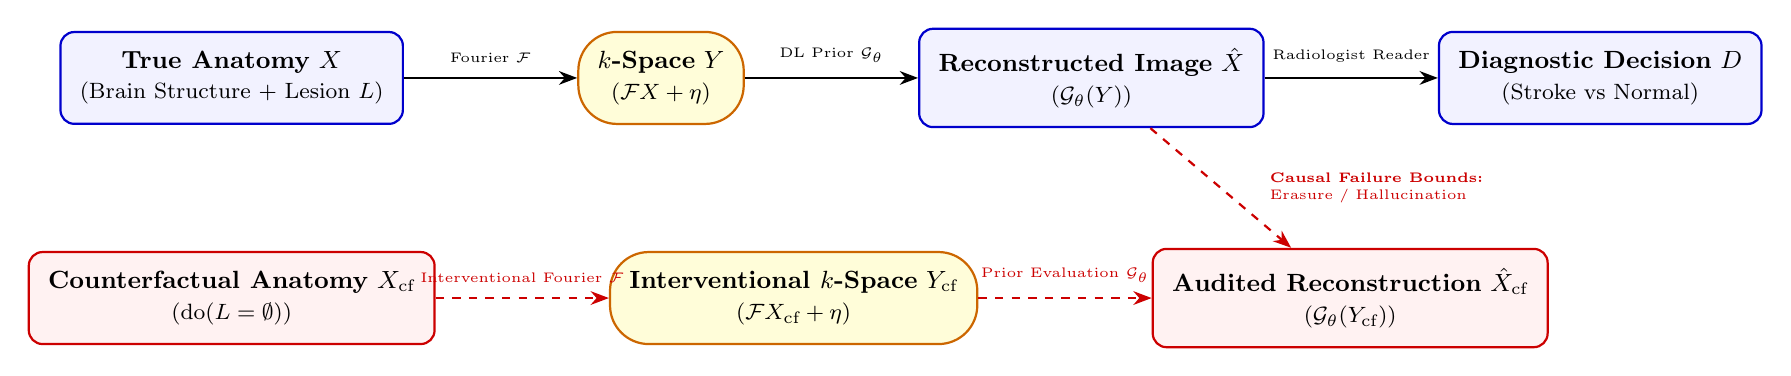
\begin{tikzpicture}[
    node distance=1.0cm and 1.6cm,
    box/.style={draw=blue!80!black, rectangle, rounded corners=5pt, fill=blue!5, thick, inner sep=7pt, align=center, font=\small, minimum height=1.1cm},
    intervent/.style={draw=red!80!black, rectangle, rounded corners=5pt, fill=red!5, thick, inner sep=7pt, align=center, font=\small, minimum height=1.1cm},
    obs/.style={draw=orange!80!black, rectangle, rounded corners=14pt, fill=yellow!15, thick, inner sep=7pt, font=\small, align=center, minimum height=1.1cm},
    arrow/.style={->, >=Stealth, thick},
    dashedarrow/.style={->, >=Stealth, thick, dashed, red!80!black}
]

% Top Row: Observational Pipeline
\node[box] (X) {\textbf{True Anatomy} $X$\\ \footnotesize (Brain Structure + Lesion $L$)};
\node[obs, right=2.2cm of X] (Y) {\textbf{$k$-Space} $Y$\\ \footnotesize ($\mathcal{F}X + \eta$)};
\node[box, right=2.2cm of Y] (Xhat) {\textbf{Reconstructed Image} $\hat{X}$\\ \footnotesize ($\mathcal{G}_\theta(Y)$)};
\node[box, right=2.2cm of Xhat] (D) {\textbf{Diagnostic Decision} $D$\\ \footnotesize (Stroke vs Normal)};

% Arrows Top Row
\draw[arrow] (X) -- (Y) node[midway, above=2pt, font=\tiny] {Fourier $\mathcal{F}$};
\draw[arrow] (Y) -- (Xhat) node[midway, above=2pt, font=\tiny] {DL Prior $\mathcal{G}_\theta$};
\draw[arrow] (Xhat) -- (D) node[midway, above=2pt, font=\tiny] {Radiologist Reader};

% Bottom Row: Counterfactual Interventional Pipeline
\node[intervent, below=1.6cm of X] (Xcf) {\textbf{Counterfactual Anatomy} $X_{\text{cf}}$\\ \footnotesize ($\mathrm{do}(L = \emptyset)$)};
\node[obs, right=2.2cm of Xcf] (Ycf) {\textbf{Interventional $k$-Space} $Y_{\text{cf}}$\\ \footnotesize ($\mathcal{F}X_{\text{cf}} + \eta$)};
\node[intervent, right=2.2cm of Ycf] (Xhatcf) {\textbf{Audited Reconstruction} $\hat{X}_{\text{cf}}$\\ \footnotesize ($\mathcal{G}_\theta(Y_{\text{cf}})$)};

% Arrows Bottom Row
\draw[dashedarrow] (Xcf) -- (Ycf) node[midway, above=2pt, font=\tiny, text=red!80!black] {Interventional Fourier $\mathcal{F}$};
\draw[dashedarrow] (Ycf) -- (Xhatcf) node[midway, above=2pt, font=\tiny, text=red!80!black] {Prior Evaluation $\mathcal{G}_\theta$};

% Interventional Comparison Arrow
\draw[dashedarrow] (Xhat) -- (Xhatcf) node[midway, right=14pt, font=\tiny, align=left, text=red!80!black] {\textbf{Causal Failure Bounds:}\\ Erasure / Hallucination};

\end{tikzpicture}%
}
\caption{Physics-Gated Causal Directed Acyclic Graph (DAG) formalizing the SCM tuple $\mathcal{M} = \langle V, U, F, P(U) \rangle$ for reference-flexible safety auditing (RQ3). In observational reconstruction (top), undersampled multi-coil $k$-space data $Y_c$ passes through neural prior $\mathcal{G}_\theta$ to produce $\hat{X}$. In counterfactual interventional stress-testing (bottom), targeted anatomical do-operators $\mathrm{do}(L = \emptyset)$ evaluate whether neural priors suppress true acute stroke penumbras or fabricate generative hallucinations under physical $k$-space data consistency constraints $\|\mathcal{F}\hat{X} - Y\|_2$.}
\label{fig:causal_dag}
\end{figure*}

Concretely, a Structural Causal Model (SCM) for physics-constrained reconstruction can be defined by the 4-tuple $\mathcal{M} = \langle V, U, F, P(U) \rangle$:
\begin{enumerate}
\item \textbf{Endogenous Variables ($V$):} $V = \{X, Y, \hat{X}, L, D\}$, where $X \in \mathbb{R}^{H \times W \times D}$ denotes true 3D patient anatomy, $Y \in \mathbb{C}^{N_c \times K}$ denotes complex multi-coil undersampled $k$-space data, $\hat{X} = \mathcal{G}_\theta(Y) \in \mathbb{R}^{H \times W \times D}$ is the deep learning reconstructed volume, $L \in \{0, 1\} \times \mathbb{R}^3$ specifies pathological lesion presence and volume (e.g., acute ischemic stroke penumbra), and $D \in \{0, 1\}$ represents the downstream diagnostic clinical decision.
\item \textbf{Exogenous Noise Variables ($U$):} $U = \{U_X, U_Y, U_{\mathcal{G}}\}$, capturing background anatomical variations ($U_X$), scanner thermal noise and $B_0$ field inhomogeneity shifts ($U_Y \sim \mathcal{CN}(0, \sigma^2 I)$), and stochastic generative noise seeds ($U_{\mathcal{G}}$).
\item \textbf{Structural Causal Functions ($F$):} The causal mechanism assignments are formulated as:
\begin{equation}
\begin{aligned}
L &:= f_L(U_X), \\
X &:= f_X(L, U_X), \\
Y_c &:= f_{Y_c}(X, U_{Y_c}) \\
&= \mathbf{M}_\Omega \mathcal{F} (S_c \cdot X) + \eta_c, \quad (c \in \{1, \dots, N_c\}), \\
\hat{X} &:= f_{\hat{X}}(Y, U_{\mathcal{G}}) = \mathcal{G}_\theta(Y, U_{\mathcal{G}}), \\
D &:= f_D(\hat{X}).
\end{aligned}
\end{equation}
\end{enumerate}

where $S_c$ denotes complex spatial receiver coil sensitivity maps for coil $c$, $\mathbf{M}_\Omega$ is the binary $k$-space undersampling trajectory mask, $\mathcal{F}$ represents the 2D/3D spatial Fourier transform operator, and $\eta_c \sim \mathcal{CN}(0, \sigma_c^2 I)$ models multi-channel complex thermal noise across the $N_c$ receiver coils. Defining the multi-coil forward encoding operator $\mathbf{A} = \mathbf{M}_\Omega \mathcal{F} \mathbf{S}$ (where $\mathbf{S} = [S_1, \dots, S_{N_c}]^T$), this multi-coil formulation grounds the physical data-consistency ($\mathcal{DC}$) operator:
\begin{equation}
\hat{X}_{\mathcal{DC}} = (\mathbf{A}^H \mathbf{A} + \lambda \mathbf{I})^{-1} (\mathbf{A}^H Y + \lambda \mathcal{G}_\theta(Y)),
\end{equation}
enforcing that multi-coil physical data consistency $\mathbf{A} \hat{X} \approx Y$ is strictly maintained across all receiver channels.

Under this SCM, observational model evaluation computes the conditional distribution $P(\hat{X} \mid Y = y) = \int P(\hat{X} \mid Y = y, u_{\mathcal{G}}) P(u_{\mathcal{G}} \mid Y = y) \, du_{\mathcal{G}}$. In contrast, counterfactual interventional safety auditing computes the interventional distribution under Pearl's Abduction-Action-Prediction framework:
\begin{equation}
\begin{aligned}
&P(\hat{X}_{Y_{\text{cf}}} \mid X=x, Y=y, \mathrm{do}(L=\emptyset)) \\
&= P\Big( \mathcal{G}_\theta\big( \mathbf{M}_\Omega \mathcal{F} (S_c \cdot f_X(\emptyset, u_X)) + \eta_c, u_{\mathcal{G}} \big) \Big),
\end{aligned}
\end{equation}
where exogenous background variables $u_X, u_Y, u_{\mathcal{G}}$ are abduced from observed patient volume $(x, y)$ and held strictly constant during counterfactual interventional simulation.

The abduction step, which infers patient-specific exogenous factors $\mathbf{u}=(u_X,u_Y,u_{\mathcal{G}})$ from the observed pair $(x,y)$, can be realized with deterministic diffusion (DDIM) inversion, VQ-VAEs, or normalizing flows \cite{peng2026latent}. Fixing abduced factors holds background anatomy invariant, so only the intervened lesion term differs. In physics-constrained diffusion solvers \cite{gungor2023adaptive,peng2026latent}, a multi-coil data-consistency ($\mathcal{DC}$) operator constrains each reverse-diffusion update:
\begin{equation}
\begin{aligned}
\mathbf{x}_{t-1} &= \mathcal{DC}\left(\mu_\theta(\mathbf{x}_t, t), Y\right) \\
&= (\mathbf{A}^H \mathbf{A} + \lambda \mathbf{I})^{-1} \left( \mathbf{A}^H Y + \lambda \mu_\theta(\mathbf{x}_t, t) \right),
\end{aligned}
\end{equation}
where $\mathbf{A}$ is the multi-coil forward encoding operator, $\mathbf{A}^H$ is its adjoint, and $\mu_\theta(\mathbf{x}_t, t)$ is the unconditional score-based diffusion model mean prediction at step $t$.

\paragraph{Posterior sampling vs.\ counterfactual intervention}
It is worth separating posterior sampling from counterfactual intervention, because the two are often conflated. Diffusion posterior sampling and its relatives draw data-consistent candidates from $p(X\mid Y)$, which quantifies epistemic uncertainty but stays observational: nothing in the sample tells you whether a missing lesion was lost to aliasing or smoothed away by the prior. A counterfactual intervention edits the structural equation $f_X$ through $\mathrm{do}(L=\emptyset)$ or $\mathrm{do}(L=v)$ with the background factors held fixed, which is what isolates the prior's effect on the lesion.

\paragraph{Null-Space Invariance Theorem for Physics Gating}
A common safety gate checks the $k$-space data-consistency residual against a tolerance, $\|\mathbf{A}\hat{X} - Y\|_2 \le \epsilon$. This gate cannot work for the failures at issue here, because the residual is unchanged by any error $\boldsymbol{\delta}$ lying in the null space $\mathcal{N}(\mathbf{A})$ of the forward operator:
\begin{equation}
\label{eq:nullspace_theorem}
\begin{aligned}
\|\mathbf{A}(\hat{X} + \boldsymbol{\delta}) - Y\|_2 &= \|\mathbf{A}\hat{X} + \mathbf{A}\boldsymbol{\delta} - Y\|_2 \\
&= \|\mathbf{A}\hat{X} - Y\|_2, \quad \forall \boldsymbol{\delta} \in \mathcal{N}(\mathbf{A}).
\end{aligned}
\end{equation}
Erased lesions and hallucinated structure both live in that unmeasured null space, which is why a residual gate detects neither. Auditing has to be done on the null-space component itself \cite{bhadra2021hallucinations,shimron2022implicit}:
\begin{equation}
\label{eq:nullspace_component}
\hat{X}_{\mathcal{N}} = (\mathbf{I} - \mathbf{A}^{+}\mathbf{A})\hat{X},
\end{equation}
where $\mathbf{A}^{+}$ denotes the pseudoinverse of the multi-coil acquisition operator. Auditing the counterfactual reconstruction $\hat{X}_{\text{cf}} = \mathcal{G}_\theta(Y_{\text{cf}})$ measures prior hallucination energy on $\hat{X}_{\mathcal{N}}$ while maintaining physical $k$-space data consistency.

\paragraph{Standardized Pre-Deployment Safety Checklist}

To translate the preceding analysis into practice, we propose a five-phase pre-deployment safety checklist for auditing AI brain MRI reconstruction (Table~\ref{tab:predeployment_checklist}). The checklist is a synthesis-informed recommendation awaiting prospective validation, not an existing regulatory instrument, and no included study evaluated it. The thresholds shown are illustrative starting points that make each phase concrete; real pass criteria must be set per application against reader-validated references, and we deliberately avoid presenting them as validated cut-offs.

\begin{table*}[t]
\centering
\caption{Proposed five-phase pre-deployment safety checklist for clinical AI brain MRI reconstruction. Thresholds are illustrative and require per-application calibration.}
\label{tab:predeployment_checklist}
\small
\setlength{\tabcolsep}{6pt}
\renewcommand{\arraystretch}{1.18}
\begin{tabular}{>{\raggedright\arraybackslash}p{0.16\textwidth} >{\raggedright\arraybackslash}p{0.24\textwidth} >{\raggedright\arraybackslash}p{0.30\textwidth} >{\raggedright\arraybackslash}p{0.24\textwidth}}
\hline
\textbf{Safety Phase} & \textbf{Core Audit Requirement} & \textbf{Mandatory Verification Metric / Protocol} & \textbf{Clinical Deployment Gate} \\
\hline
Phase 1: Inverse Problem Physics & Verification of physical multi-coil $k$-space data consistency ($\mathcal{DC}$) operator and raw data access. \emph{Certifies measurement-space fidelity only: by construction this gate is blind to edits in the null space of $\mathbf{A}$, which is why Phases 2--3 are required and not optional.} & Relative multi-coil $k$-space residual norm $\|\mathbf{A}\hat{X} - Y\|_2 / \|Y\|_2 \le \epsilon$ ($\epsilon < 0.01$) on un-normalized raw data & Pass: Normalized $k$-space data consistency error $< 1.0\%$ across all channels; un-normalized raw $k$-space access verified. Passing this phase alone is \emph{not} a safety claim. \\
\hline
Phase 2: Lesion-Preservation Stress-Test & Counterfactual lesion stress-testing under targeted intervention $\mathrm{do}(L = v)$ & Lesion ROI contrast-to-noise ratio drop $\Delta \text{CNR} \le 5\%$ and volume error $|V_{\hat{X}} - V_X| / V_X \le 0.02$ & Pass: Lesion recall $\ge 98.0\%$ and lesion volume deviation $< 2.0\%$ on DWI/FLAIR. \\
\hline
Phase 3: Hallucination \& OOD Audit & Null-space audit of prior-supplied content $(\mathbf{I}-\mathbf{A}^{+}\mathbf{A})\hat{X}$, epistemic uncertainty mapping $\text{Var}_{p(X|Y)}(\hat{X})$, and OOD perturbation stress-testing & Null-space energy $\|(\mathbf{I}-\mathbf{A}^{+}\mathbf{A})\hat{X}\|_2$ localized and reviewed wherever it overlaps a candidate lesion; OOD hallucinated feature count $N_{\text{false}} = 0$; epistemic variance bound $\sigma^2_{\text{epistemic}} \le \tau_{\text{bg}}$ & Pass: Zero false-positive generative structures ($N_{\text{false}}=0$) under distribution shift, with null-space content attributable to the prior rather than to the measurement. \\
\hline
Phase 4: Reader / Learned-Metric Evaluation & Task-based radiologist reader study and MRI-specific learned perceptual assessment & Diagnostic Acceptability Likert score $\ge 4.0/5.0$ and non-inferiority ROC margin $\Delta \text{AUC} \le 0.02$ vs reference & Pass: Mean radiologist diagnostic Likert score $\ge 4.0/5.0$ and reader agreement $\kappa \ge 0.75$. \\
\hline
Phase 5: Multi-Site Robustness Audit & Multi-site, cross-vendor scanner hardware ($1.5\text{T}, 3\text{T}, 7\text{T}$) generalizability audit & Cross-site performance degradation $\Delta \text{PSNR}_{\text{site}} \le 0.5\text{ dB}$ and zero contrast inversion & Pass: Cross-vendor diagnostic score drop $\le 3.0\%$ across $1.5\text{T}, 3\text{T}, 7\text{T}$ platforms. \\
\hline
\end{tabular}
\end{table*}

\subsection{Limitations and Threats to Validity}
\label{sec:validity}

\textit{a) Construct validity.} The question here is whether what we measured corresponds to reconstruction safety and diagnostic fidelity at all. We searched with broad, high-sensitivity terms for architectures, artifacts, and evaluation paradigms, and the resulting corpus does span the reconstruction-safety literature, covering pixel-wise metrics, perceptual losses, and reader studies across 220 studies. What it cannot do is guarantee that a given metric means the same thing wherever it appears. Studies differ in what they treat as the quantity of interest, so a rank correlation with reader scores in one paper is not straightforwardly the same measurement as in another, and grouping such values under one heading is an interpretation we are making, not a property of the data.

\textit{b) Internal validity.} A protocol fixed before screening began, a documented search across seven digital libraries, and independent screening against explicit PICOS criteria by three reviewers give reasonable protection here, and every extracted value is released with the verbatim snippet supporting it, so any assignment can be checked against its source. Two threats survive that. Retrieval failed for 422 of the 1{,}149 candidate reports even after a post-registration open-access retrieval round (9 embargoed in PubMed Central until 2026--2027, 1 title not licensed to our institution, 1 with no locatable accessible copy, and 411 with no open-access copy and no subscription access); those reasons are structural rather than selective, but we cannot show that the records we could not obtain resemble the ones we could. And 18 of the 220 included studies were assessed on title, abstract, and controlled vocabulary alone, with a further 2 on partial text, because no complete full text could be obtained; for those the extracted values rest on a narrower evidentiary base, which the released per-study file records explicitly so that any reader can see which studies are affected.

\textit{c) External validity.} The corpus covers $1.5\text{T}$, $3\text{T}$, and $7\text{T}$, several vendors' coil configurations, and the major pulse sequences, which gives it reasonable clinical reach. Against that, reconstruction tasks, acquisition protocols, architectures, datasets, validation strategies, and evaluation metrics all vary substantially, and that variation is why we report the direction and consistency of findings instead of their magnitudes. Many algorithmic studies use retrospectively undersampled single-center data, which flatters performance relative to prospective multi-center use; the smaller prospective reader-study subset \cite{bash2021deep,radmanesh2022exploring} generalizes more directly. Publication bias cannot be excluded either. Improved performance and favourable metrics are easier to publish than failed approaches, failure cases, and clinically relevant errors. For a review about failure modes this cuts close: our corpus comes from a literature with little incentive to report the very thing we are studying. We ran no funnel-plot or small-study asymmetry test, which the absence of a common effect measure rules out in any case.

\textit{d) Conclusion validity.} Since pixel-wise metrics agree only loosely with radiologist judgement (RQ1), a primary study resting on PSNR and SSIM alone supports a safety claim less well than one with reader studies or uncertainty-aware observers, and we weight the evidence accordingly. Three further constraints bound what we can claim. We applied no formal certainty framework such as GRADE or CERQual: the included studies report algorithmic development rather than controlled clinical interventions, and the domains those instruments assess do not map onto that literature. No finding here therefore carries a graded certainty rating. We also performed no meta-analysis, because the heterogeneity described above prevents reliable pooling, and pooling incommensurable quantities would produce a precision the evidence does not possess. Every number we give is a result from a named study rather than a summary estimate. This review should be read as a structured qualitative synthesis that identifies evaluation limitations and safety gaps, and no range we quote should be read as an interval estimate.

% =============================================================================
\section{Conclusion}
\label{sec:conclusion}
% =============================================================================

We reviewed 220 primary studies on the safety, artifacts, and fidelity of deep-learning and accelerated brain MRI reconstruction. Three things came out of it. Conventional fidelity metrics track radiologist diagnostic judgement poorly, and the evaluations that would expose the gap, reader studies above all, are reported in a small minority of the literature (RQ1). The reason is structural rather than incidental: background voxels average focal error away, the loss functions are sign-symmetric where diagnosis is not, adversarial terms pay for invented texture, and every one of these metrics assumes a registered reference that patient motion destroys (RQ2). And no evaluation paradigm now in use settles the safety question by itself, which is what the paradigm-by-paradigm synthesis under RQ3 makes explicit. The specific vulnerabilities matter as much as the aggregate picture. High PSNR and SSIM coexist with erased $1\text{--}3\text{ mm}$ cerebral microbleeds on SWI, with inter-slice step discontinuities in 3D volumes, and with features leaking between contrasts in multi-sequence networks. Closed vendor software compounds this by withholding the raw $k$-space that independent auditing would require. On the basis of those gaps, and separately from them, we propose a physics-grounded structural causal framework and a five-phase pre-deployment checklist as a roadmap for future benchmarking and audit design. Neither has been prospectively validated; both are proposals rather than findings. What the evidence itself supports is narrower and firmer: evaluation instruments must become sensitive to focal diagnostic change, and raw data must become accessible, or reconstruction models will continue to be certified by numbers that cannot see how they fail.

% =============================================================================
% Back-Matter Disclosures & Statements
% =============================================================================

\section*{Data and Code Availability}
The search and retrieval scripts (utilizing the PubMed E-utilities API, IEEE Xplore REST API, Scopus API, Web of Science API, SpringerLink API, OpenAlex API, and Semantic Scholar API), along with deduplicated corpus metadata and screening decision logs, are deposited on the Open Science Framework at \url{TODO-INSERT-OSF-DOI}. The deposit is organised in six components. \emph{Manuscript}: the compiled article and its LaTeX source. \emph{Protocol and registration}: the review protocol written before screening began (\texttt{protocol.json}), the executed search strategy (\texttt{search\_strategy.json}), the operational screening criteria (\texttt{ie\_criteria.yaml}), the protocol reported against PRISMA-P, the search against PRISMA-S, the eligibility criteria, the data extraction form, the appraisal plan, a log of deviations from the protocol, and the three reviewer sign-off worksheets together with the script that merges them. \emph{PRISMA}: \texttt{PRISMA\_flow\_report.json} and \texttt{prisma\_log.json}, detailing the multi-stage deduplication and screening counts, with per-database identification counts and the completed PRISMA 2020 checklist. \emph{Included studies}: \texttt{included\_characteristics.csv}, giving extracted characteristics for all 185 included studies; \texttt{included\_characteristics\_supplement.csv}, the per-study quality appraisal with the verbatim quotation supporting each rating; the raw QUADAS-2 worksheets those ratings were drawn from; a data dictionary; and \texttt{included\_studies\_185.bib}. \emph{Screening decisions}: every title/abstract and full-text decision with its recorded reason, including the post-registration second screening round (\texttt{fulltext\_screening\_decisions\_round2.csv}), and a data dictionary for the decision files. \emph{Code}: the scripts that build and verify the per-study release files. The deposit is retrospective and is described as such in its documentation. Full-text PDFs of the included studies are not redistributed, because publisher licence terms do not permit it; the DOI list in \texttt{included\_studies\_220.bib} identifies the corpus in full.

The same materials, together with the analysis code, are mirrored at \url{https://github.com/dmai287/brain-mri-recon-safety-slr}. All results reported in this paper correspond to the archived release \texttt{v1.0.0} of that repository, commit \texttt{<COMMIT-SHA>}, deposited at Zenodo under DOI \texttt{<10.5281/zenodo.XXXXXXX>}; readers should cite the archived release rather than the mutable repository, and the tagged commit is the reference against which every number in this paper can be regenerated. Screening was performed by three reviewers (authors DTM, TVP, and TNTD) working independently, with consensus adjudication of \emph{flagged} records; included studies were verified against the fullest text obtainable, which was complete full text for 200 of the 220.

\section*{Ethics Approval and Consent to Participate}
This review synthesizes secondary data from published, de-identified study corpora. It involved no human participants, no animal experimentation, and no collection of private health data, so institutional review board approval and patient informed consent were not required.

\section*{Declaration of Competing Interest}
The authors declare that they have no known competing financial interests, commercial affiliations, or personal relationships that could have appeared to influence the work reported in this paper.

\section*{Funding Statement}
This research was supported by institutional research computing infrastructure and scholarship funding from RMIT University. The funder had no role in the design of the review, the search strategy, the eligibility criteria, the screening or appraisal of studies, the synthesis or interpretation of findings, the writing of this report, or the decision to submit it for publication. No external, commercial, or industry funding was received, and no vendor of MRI hardware or reconstruction software contributed financial or non-financial support to this work.

% Supplementary Table S1: the 220 included studies (PRISMA 2020 item 17).
% Move this \input to a separate supplementary document if the journal prefers.
\input{supplementary_table_s1}

\bibliographystyle{IEEEtran}
\bibliography{ref2}

\end{document}

